%%%%%%%%%%%%%%%%%%%%%%%%%%%%%%%%%%%%%%%%%%%%%%%
%%% Template for lab reports used at STIMA
%%%%%%%%%%%%%%%%%%%%%%%%%%%%%%%%%%%%%%%%%%%%%%%

%%%%%%%%%%%%%%%%%%%%%%%%%%%%%% Sets the document class for the document
% Openany is added to remove the book style of starting every new chapter on an odd page (not needed for reports)
\documentclass[10pt,english, openany]{book}

%%%%%%%%%%%%%%%%%%%%%%%%%%%%%% Loading packages that alter the style
\usepackage{graphicx}
\usepackage{subcaption}
\usepackage[]{color}
\usepackage{alltt}
\usepackage[T1]{fontenc}
\usepackage[utf8]{inputenc}
\usepackage{amsfonts}
\usepackage{amsmath}
\setcounter{secnumdepth}{2}
\setcounter{tocdepth}{2}
\usepackage[titletoc]{appendix}
\setlength{\parskip}{\smallskipamount}
\setlength{\parindent}{0pt}

% Set page margins
\usepackage[top=100pt,bottom=100pt,left=68pt,right=66pt]{geometry}

% Prevents LaTeX from filling out a page to the bottom
\raggedbottom

% Adding both languages
\usepackage[english, italian]{babel}

% All page numbers positioned at the bottom of the page
\usepackage{fancyhdr}
\fancyhf{} % clear all header and footers
\fancyfoot[C]{\thepage}
\renewcommand{\headrulewidth}{0pt} % remove the header rule
\pagestyle{fancy}

% Changes the style of chapter headings
%\usepackage{titlesec}
% \usepackage[Glenn]{fncychap}
% Adds table captions above the table per default
\usepackage{float}
\floatstyle{plaintop}
\restylefloat{table}

% Adds space between caption and table
\usepackage[tableposition=top]{caption}

% Adds hyperlinks to references and ToC
\usepackage{cite}
\usepackage{hyperref}
%\hypersetup{hidelinks,linkcolor = black} % Changes the link color to black and hides the hideous red border that usually is created

% If multiple images are to be added, a folder (path) with all the images can be added here 
\graphicspath{ {Figures/} }

% Separates the first part of the report/thesis in Roman numerals
\frontmatter

% Algorithms
\usepackage[ruled,vlined]{algorithm2e}


%%%%%%%%%%%%%%%%%%%%%%%%%%%%%% Starts the document
\begin{document}

%%% Selects the language to be used for the first couple of pages
\selectlanguage{english}

\author{Julian Eßer}
\title{Comparison of Optimal Control Frameworks in the Context of Bipedal Walking}

%%%%% Adds the title page
\begin{titlepage}
\maketitle
\end{titlepage}

% Adds a table of contents
\tableofcontents{}

%%%%%%%%%%%%%%%%%%%%%%%%%%%%%%%%%%%%%%%%%%%%%%%%%%%%%%%%%%%%%%%%%%%%%%%%%%%%%%%%%%%%%%%%%%%%
%%%%%%%%%%%%%%%%%%%%%%%%%%%%%%%%%%%%%%%%%%%%%%%%%%%%%%%%%%%%%%%%%%%%%%%%%%%%%%%%%%%%%%%%%%%%
%%%%% Text body starts here!
\mainmatter
\chapter{INTRODUCTION}
\textbf{Project Objectives}

The primary goal of this two-month project is to gain insights about the bipedal walking capabilities of two open-source frameworks for optimal control of robots (Crocoddyl, Drake).

\textbf{In particular, this involves}
\begin{enumerate}
\item Installing and familiarizing with the libraries description of dynamical systems and optimization problems,
\item Working with the provided examples, especially those related to legged-locomotion,
\item Integrating a universal description of the RH5 robot and test the solvers 
\item Comparing the frameworks in terms of suitability for performing bipedal walking tasks.
\end{enumerate}

\textbf{Organisation}

All tasks related to this project are handled as issues and managed centrally from the \textbf{related repository} \cite{julesserOCFrameworks}.
Even though most of the implementation  is done in the forked repositories of the according frameworks, this seems to be a clear way of organizing.   

\chapter{CROCODDYL - LAAS-CNRS}\label{chapter1}
\section{Introduction}
\subsection{Motivation}
Crocoddyl is an \textbf{optimal control library for robot control under contact sequence}. Its solver is based on an efficient Differential Dynamic Programming (DDP) algorithm. Crocoddyl computes optimal trajectories along with optimal feedback gains. It uses Pinocchio for fast computation of robot dynamics and its analytical derivatives \cite{crocoddylweb}. 

Crocoddyl is focused on multi-contact optimal control problem (MCOP) which has the form:

$$\mathbf{X}^*,\mathbf{U}^*=
\begin{Bmatrix} \mathbf{x}^*_0,\cdots,\mathbf{x}^*_N \\
				  \mathbf{u}^*_0,\cdots,\mathbf{u}^*_N
\end{Bmatrix} =
\arg\min_{\mathbf{X},\mathbf{U}} \sum_{k=1}^N \int_{t_k}^{t_k+\Delta t} l(\mathbf{x},\mathbf{u})dt$$
subject to
$$ \mathbf{\dot{x}} = \mathbf{f}(\mathbf{x},\mathbf{u}),$$
$$ \mathbf{x}\in\mathcal{X}, \mathbf{u}\in\mathcal{U}, \boldsymbol{\lambda}\in\mathcal{K}.$$
where
\begin{itemize}
\item the state $\mathbf{x}=(\mathbf{q},\mathbf{v})$ lies in a manifold, e.g. Lie manifold $\mathbf{q}\in SE(3)\times \mathbb{R}^{n_j}$, $n_j$ being the number of degrees of freedom of the robot.
\item the system has underactuacted dynamics, i.e. $\mathbf{u}=(\mathbf{0},\boldsymbol{\tau})$,
\item $\mathcal{X}$, $\mathcal{U}$ are the state and control admissible sets, and
\item $\mathcal{K}$ represents the contact constraints.
\end{itemize}

Note that $\boldsymbol{\lambda}=\mathbf{g}(\mathbf{x},\mathbf{u})$ denotes the contact force, and is dependent on the state and control.

\subsection{Features}
According to the description in the Github repository \cite{crocoddylweb}, it comprises the following features:

Crocoddyl is \textbf{versatible}:
\begin{itemize}
\item various optimal control solvers (DDP, FDDP, BoxDDP, etc) - single and multi-shooting methods
\item analytical and sparse derivatives via Pinocchio
\item Euclidian and non-Euclidian geometry friendly via Pinocchio
\item handle autonomous and nonautomous dynamical systems
\item numerical differentiation support
\end{itemize}

Crocoddyl is \textbf{efficient} and \textbf{flexible}:
\begin{itemize}
\item cache friendly,
\item multi-thread friendly
\item Python bindings (including models and solvers abstractions)
\item C++ 98/11/14/17/20 compliant
\item extensively tested
\end{itemize}



\section{How-To}
\subsection{Install}
\subsubsection{Two ways to go}
Basically there are existing two ways of installing Crocoddyl: 
\begin{itemize}
\item Option 1: Installation via the \textit{robotpkg } package manager
\item Option 2: Installation from source
\end{itemize} 
I personally would recommend the installation through \textit{robotpkg}, since it preserves you from dealing with the multiple dependencies of Crocoddyl and therefore seems to be the faster approach. Generally you should decide beforehand which python version you want to use. This effects the robotpkg version as well as the export of the PYTHONPATH variable. 

\subsubsection{Installation via robotpkg (preferred)}
Steps for installing via robotpkg according to the installation section of \cite{crocoddylweb}
\begin{enumerate}
	\item Add robotpkg as source repository to apt:
	\begin{verbatim}
	sudo tee /etc/apt/sources.list.d/robotpkg.list <<EOF
	deb [arch=amd64] http://robotpkg.openrobots.org/wip/packages/debian/pub $(lsb_release -sc) robotpkg
	deb [arch=amd64] http://robotpkg.openrobots.org/packages/debian/pub $(lsb_release -sc) robotpkg
	EOF
	\end{verbatim}
	\item Register the authentication certificate of robotpkg:
	\begin{verbatim}
	curl http://robotpkg.openrobots.org/packages/debian/robotpkg.key | sudo apt-key add -
	\end{verbatim}
	\item You need to run at least once apt update to fetch the package descriptions:
	\begin{verbatim}
	sudo apt-get update
	\end{verbatim}
	\item The installation of Crocoddyl:
	\begin{verbatim}
	sudo apt install robotpkg-py27-crocoddyl # for Python 2
	sudo apt install robotpkg-py36-crocoddyl # for Python 3
	\end{verbatim}
	\item Finally you will need to configure your environment variables (watch out for the python version!), e.g.:
	\begin{verbatim}
	export PATH=/opt/openrobots/bin:$PATH
	export PKG_CONFIG_PATH=/opt/openrobots/lib/pkgconfig:$PKG_CONFIG_PATH
	export LD_LIBRARY_PATH=/opt/openrobots/lib:$LD_LIBRARY_PATH
	export PYTHONPATH=/opt/openrobots/lib/python3.6/site-packages:$PYTHONPATH
	\end{verbatim}
\end{enumerate}

\subsubsection{(Installation from source)}
If you prefer installing Crocoddyl from source, the following steps should do the work:
\begin{verbatim}
git clone https://github.com/loco-3d/crocoddyl.git 
git submodule update --init
mkdir build && cd build
export PKG_CONFIG_PATH=/opt/openrobots/lib/pkgconfig
cmake -DCMAKE_INSTALL_PREFIX=/opt/openrobots  ..
make
sudo make install
\end{verbatim}
Additionally you will have to install the dependent libraries (i.e. pinocchio, example-robot-data (optional for examples, install Python loaders), gepetto-viewer-corba (optional for display), jupyter (optional for notebooks) and matplotlib (optional for examples) and fix the incude paths.

\subsubsection{For Displaying Results: Additionally Install Gepetto-Viewer}
In order to see not just 2-dimensional plots, but also observe the 3D robot behaviour, you additionally have to install the gepetto-viewer.
\begin{verbatim}
 sudo apt install robotpkg-py36-qt4-gepetto-viewer-corba
\end{verbatim}

\subsection{Running the Examples}
Since the installation through robotpkg did not provide you with the examples from the git repository, you should clone the repo \cite{crocoddylweb} for getting the data. You do not have to build the library, since it already is installed. 
In the cloned repository go to \textit{/examples}. For running e.g. the bipedal walking example, just type
\begin{verbatim}
python3 bipedal_walk.py
\end{verbatim}
and you will see the calculations for optimal gait trajectories running in the console. 
The examples provide a \textit{plot} and \textit{display} argument. In order to display the 3D results and also plot some data, just do 
\begin{verbatim}
gepetto-gui
\end{verbatim}
for starting the 3D environment.
Then, in another terminal, run the example:
\begin{verbatim}
python3 bipedal_walk.py display plot
\end{verbatim}



\section{Abstract Workflow}
For each node (i.e. each timestep) of the optimal control problem, 
\begin{enumerate}
\item Load robot data (URDF, SRDF, Meshes)
\item Define Action Models (Dynamics+Costs) for running and terminal states 
	\begin{itemize}
	\item Setup a cost model
	\item Add the desired cost functions (state, control, frame-placement etc.)
	\item Calculate Integrated \& Differential Action Model (IAM/DAM) based on the model
	\end{itemize}
\item Define the optimal control problem (knots+IAMs, initPose)
\item Solve the Shooting Problem
\end{enumerate}



\section{Issues and Insights}
\subsection{Issues Encountered}
Since Crocoddyl currently is under active development, there frequently will occure smaller incompatibilities because of versioning issues.This is a brief overview of emerged difficulties:
\begin{itemize}
\item Python versioning errors in the examples. 

The examples most often are written for python2, which means that if you are under python3, you will have to adapt some commands (e.g. lists handling, matplotlib, print).
\item Crocoddyl versioning errors in the examples. 

Since Crocoddyl depends on other libraries (i.e. Pinnochio, example\_robot\_data), there sometimes occured errors with the class because they were not updated. 
\item Confusions displaying the results via the Gepetto-Viewer

The Gepetto-Viewer is used for displaying the robots and resulting trajectories from optimization. The examples only contain out of the box solutions. If one wants to simply display a robot in some specified pose (e.g. the initial pose) the following, quite unintuitive, commands have to be applied:
\begin{verbatim}
display = crocoddyl.GepettoDisplay(rh5_legs, 4, 4, frameNames=[rightFoot, leftFoot])
display.display(xs=[x0])
\end{verbatim}
\end{itemize}

\subsection{Cost Functions}
Notes:
\begin{itemize}
\item The cost function can contain multiple \textit{cost items} (i.e state/control error, frame displacements or center of mass tracking).
\item Weights are considered in the costs via scalar multiplication with the identity matrices (Ix, Ixx etc.) of the according cost item. 
\item These weighted matrices of cost items are simply summed up within a \textit{costModelContainer}.
\end{itemize}

\subsection{Joint Limits}
\begin{itemize}
\item Input Data: Within the URDF file, for each joint there are specified the
\begin{itemize}
	\item torque limit (effort),
	\item position limits (lower, upper),
	\item velocity limit.
\end{itemize}
\item These limits are not automatically taken into account in Crocoddyl when solving a shooting problem, but explicitly have to be adressed.
\item \textbf{Torque Limits}: Require the use of specific solvers, standard ddp is not sufficient. Implemented solvers that can handle torque limits explicitly are: 
\begin{itemize}
\item BoxDDP (Compare Tassa method \cite{tassa2014control})
\item BoxFDDP (Novel solver that is under development at LAAS)
\end{itemize}
\textbf{State Limits (Pos/Vel)}: Position and Velocity limits can be handled via penalization, i.e. added as cost terms to the optimization problem.  
\end{itemize}

\subsection{Introduction: Bipedal Walking in Crocoddyl}
\begin{itemize}
\item A long walk consists of multiple gaitphases, each phase is a single shooting problem.
\item These problems are generated with \textit{createWalkingProblem()} involving one left and one right foot step.
\item Each shooting problem contains various locomotion phases
	\begin{itemize}
	\item Double support at beginning (both legs on ground) via \textit{createSwingFootModel()}
	\item Right step (Swing-up and swing-down phase equally distributed) init via    	\textit{createFootstepModels()}
	\item Double support again
	\item Left step
	\end{itemize}	
\item In the end, all knots of all phases are basically one \textit{swingFootModel}. They only vary in the adressed foot, and if a CoM task or a swingFootTask is set.
\item The \textit{swingFootModel} is an IAM containing a 
	\begin{itemize}
	\item 6D multi-contact model,
	\item Cost model (CoM position tracking, contact friction cone, foot placement) and
	\item Differentiation (DAM) and Integration (IAM) routines.
	\end{itemize}
\end{itemize}

\subsection{Multi-Contact Model}
\subsubsection{Previous: Assume foot to have a point contact}
\begin{itemize}
\item Each \textit{swingFootModel}, meaning each knot of the OC, includes at least one individual contact model.
\item The number of contact models depends is specified via \textit{supportFootIds}, i.e. the number of foots that currently are not in the air (e.g. biped: 1 for swing-phase, 2 for double-support).
\item For each point of one foot that actually does touch the ground, a contact has to be added to the according contact model (specified via frame ID)
\item In the bipedal examples they assume a point-contact, i.e. adding only one contact per supporting foot.
\item The point-contact is specified via the name of the according link from the URDF.
\end{itemize}
\subsubsection{Extension: Consider 4 point contact per foot}
\begin{itemize}
\item Each contact model for one supporting foot now contains four contact items instead of one
\item The cost model contains now four cost items for the four friction cones instead of just one

\item The 
\end{itemize}



\section{Working with the Examples}
This section contains a brief overview of some of the examples that have been modified. Please note that many \textbf{additional explanations have been added in the commentaries of the examples}. All figures and additionaly videos are contained within the /media directory of the repo \cite{julesserOCFrameworks}. 

As stated in the ReadMe of the Repo, Crocoddyl comes with some introductory examples that are written as Jupyter notebooks (.ipynb). While 
\begin{verbatim}
examples/notebooks/introduction_to_crocoddyl.ipynb
\end{verbatim}
offers a more conceptual overview about crocoddyl, other ones represent basic underactuated systems (e.g. Cartpole swing-up, Bipdeal Walking).

\subsection{Manipulator: Multi-Point Trajectory}
The task in the tutorial
\begin{verbatim}
examples/notebooks/arm_manipulation.ipynb
\end{verbatim}
was to find an optimal trajectory for a manipulator from an initial configuration to a target point (red ball). 
\subsubsection{Extending the Example}
I extended this example to a multi-point optimal control problem by considering four targets to reach in a row. This extended example can be found in 
\begin{verbatim}
/examples/arm_manipulation_trajectory.py
\end{verbatim}
Differences to the existing one-target example include:
\begin{itemize}
\item Defining an array of the four targets in space
\item Setup individual cost functions for each of the sequences
\item Setup running and terminal models for the sequences and finally
\item Define the shooting problem as row of these sequences 
\item Optimize the weights of the cost functions successively for the four sequences.
\end{itemize}
\subsubsection{Results: Multiple Targets}
\begin{figure}[h!]
\centering
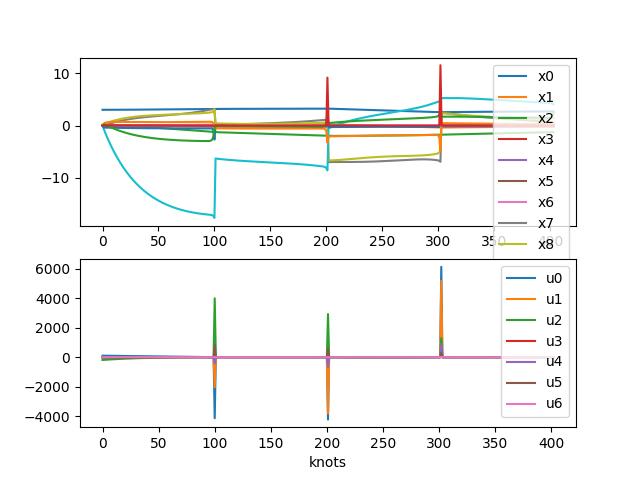
\includegraphics[width=.5\linewidth]{Media/Crocoddyl/ExArm/ArmSolution.png}
\caption{Multi-Point Optimal Control of the Manipulator for reaching four targets. The high-control peaks could be handled by a more advanced solver (e.g. box-ddp), but were not performed here.}
\end{figure}

\subsection{Talos Legs: Bipedal Walking}
The Crocoddyl library offers an example for bipedal walking with the lower body of the Talos \cite{stasse2017talos} Robot. The results of the solved trajectory can be found in Figure \ref{fig:TalosGait}. 

\begin{figure}[h!]
\centering
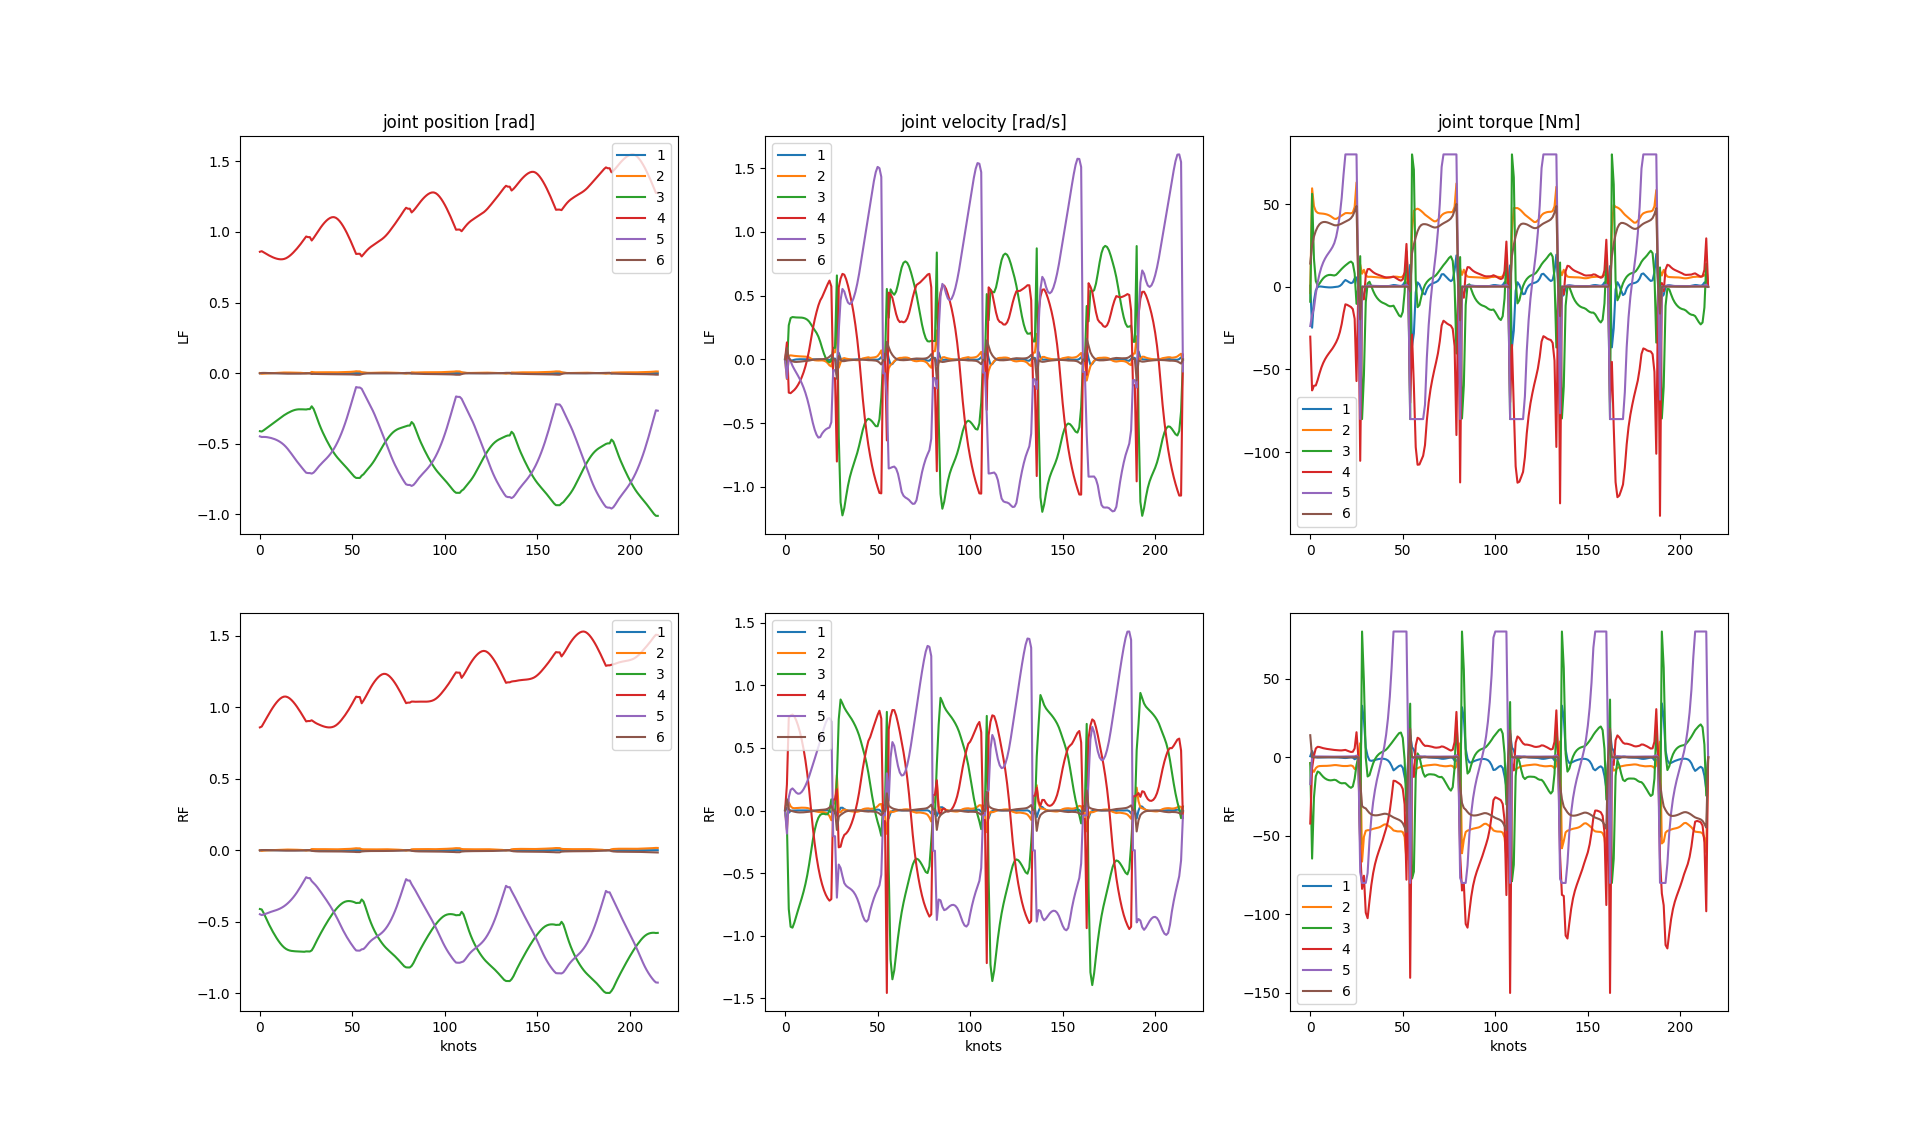
\includegraphics[width=.7\linewidth]{Media/Crocoddyl/ExBiped/TalosGait_Solution.png}
\caption{Results for a walk with three gait-phases.}
\label{fig:TalosGait}
\end{figure}

  



\section{RH5 Results}
Please note once again that all related plots and additional videos can be found in high-quality in the related github repository \cite{julesserOCFrameworks} of this project.
\subsection{Navigating the Files}
The main file for testing RH5 offers several options for setting up, analyzing and constraining the optimization problem of bipedal walking including
\begin{itemize}
\item Choosing a desired URDF 
\item Specifying gait length and variations in step length/height
\item Vary the initial pose of the robot
\item Constraining the torque input (Use different solver)
\item Defining singular or multiple point contacts per foot (Use different class from biped utils)
\end{itemize}

\subsection{Integration of the RH5 Legs into Crocoddyl}
The main issue that had to be solved was related to the underlying URDF file of the robot. In particular: 
\begin{itemize}
\item Choosing one of our several files (abstract-smurf)
\item Cutting out everything apart from the legs and the root joint
\item Fixing the mesh file paths: 

We usually define the path relative to the URDF file location, e.g.
\begin{verbatim}
"../meshes/stl/RH5_Root_Link.001.stl".
\end{verbatim}
The integrated URDF parser in Crocoddyl instead, expects the path specified via the package URI, e.g. 
\begin{verbatim}
"package://abstract-smurf/meshes/stl/RH5_Root_Link.001.stl".
\end{verbatim}
\item Adjust the contact frames for the Walking Problem.
\end{itemize}

\subsection{Performing two Steps}
Results are shown in Figure \ref{fig:rh5_two_steps}.
\begin{figure}[h!]
\centering
\begin{subfigure}{.4\textwidth}
  \centering
  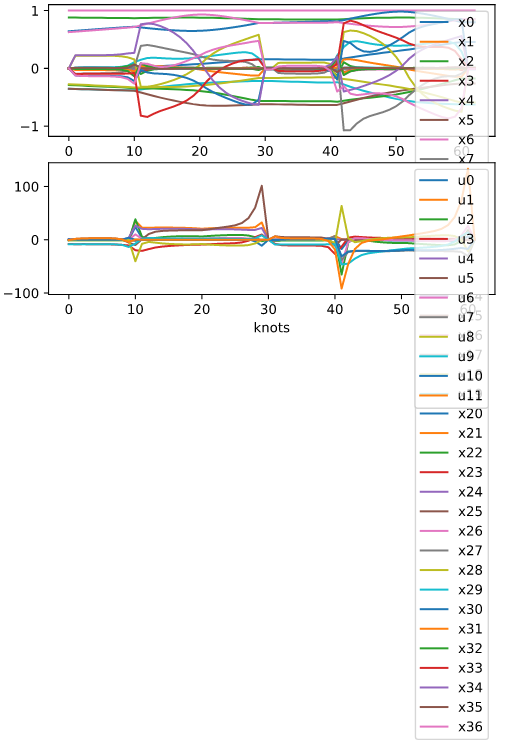
\includegraphics[width=1\linewidth]{Media/Crocoddyl/RH5/2Steps/RH52Steps_Solution.png}
  \caption{Optimal Trajectory and Conrol Inputs}
\end{subfigure}%
\begin{subfigure}{.4\textwidth}
  \centering
  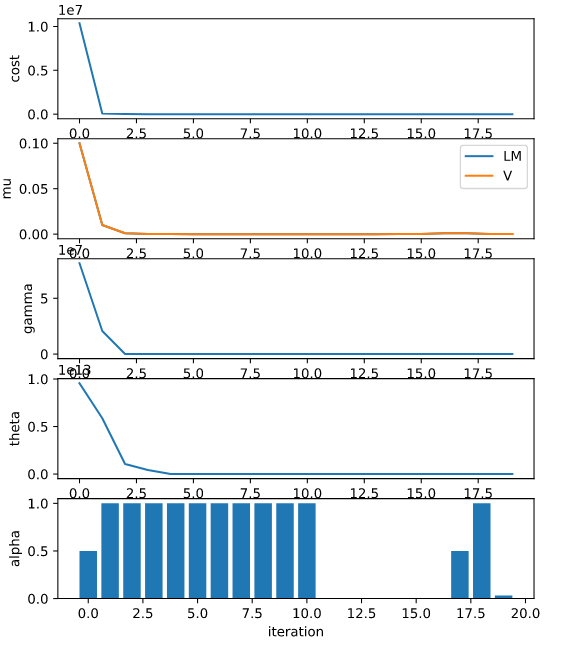
\includegraphics[width=1\linewidth]{Media/Crocoddyl/RH5/2Steps/RH52Steps_Convergence.png}
  \caption{Convergence of Solution}
\end{subfigure}
\caption{Results for a solved shooting problem defining two steps.}
\label{fig:rh5_two_steps}
\centering
\end{figure}

\subsection{Performing a Full Gait}
Results for a full gait (6 consecutive steps) are shown in Figure \ref{fig:rh5_full_gait}.
\begin{figure}[h!]
\centering
\begin{subfigure}{.8\textwidth}
  \centering
  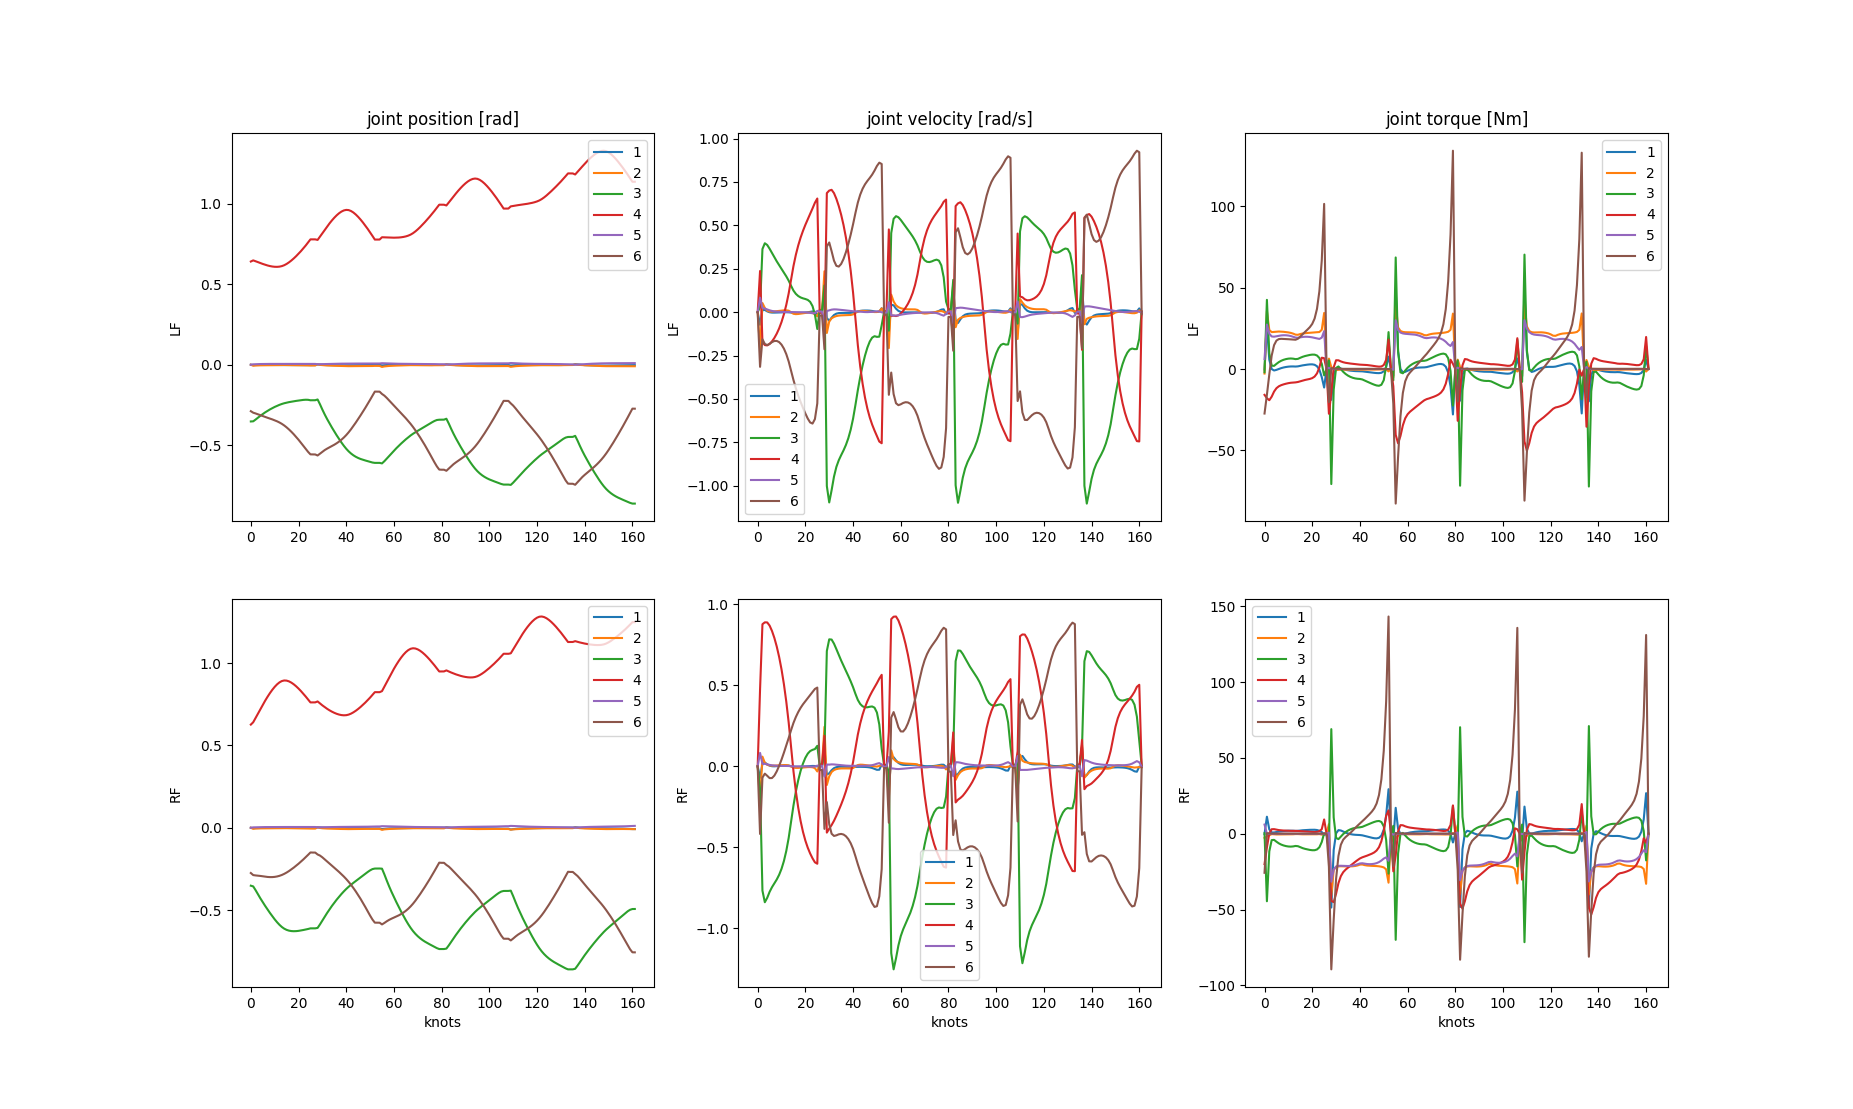
\includegraphics[width=1\linewidth]{Media/Crocoddyl/RH5/RH5Gait_Solution.png}
  \caption{Solution for states and torques.}
\end{subfigure}
\begin{subfigure}{.8\textwidth}
  \centering
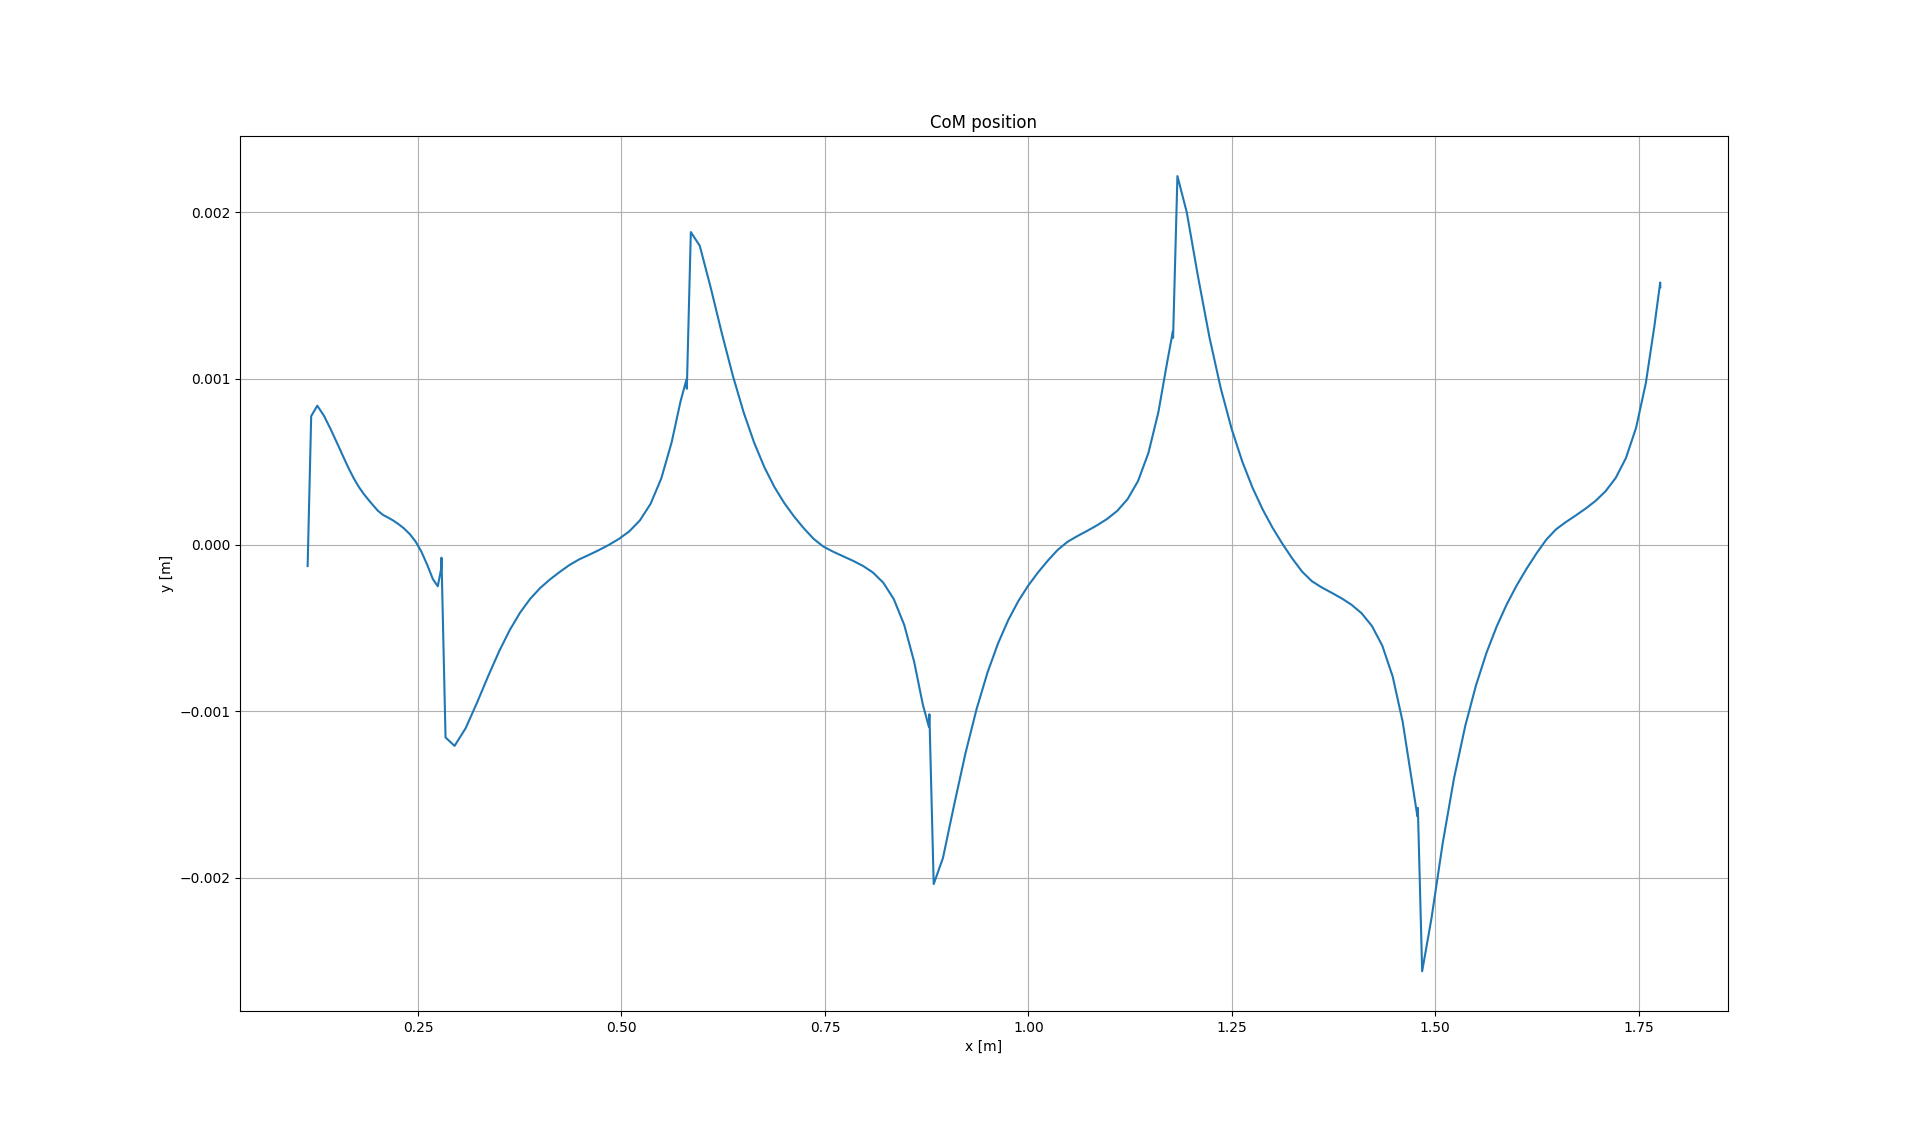
\includegraphics[width=1\linewidth]{Media/Crocoddyl/RH5/RH5Gait_CoM.png}
\caption{CoM results.}
\end{subfigure}
\caption{Results for a walk with three gait-phases. The walk is implemented as a sequence of three  consecutive shooting problems similar to the 2 steps task.}
\label{fig:rh5_full_gait}
\centering
\end{figure}

\subsection{Torque-Constrained Full Gait}
It is possible to constrain the input torques via the limits that are parsed from the URDF. However, the correct solver (box-ddp) needs to be applied to the OC problem for considering these limits.  Results are shown in Figure \ref{fig:rh5_constrain_torque}
\begin{figure}[h!]
\centering
\begin{subfigure}{.8\textwidth}
  \centering
  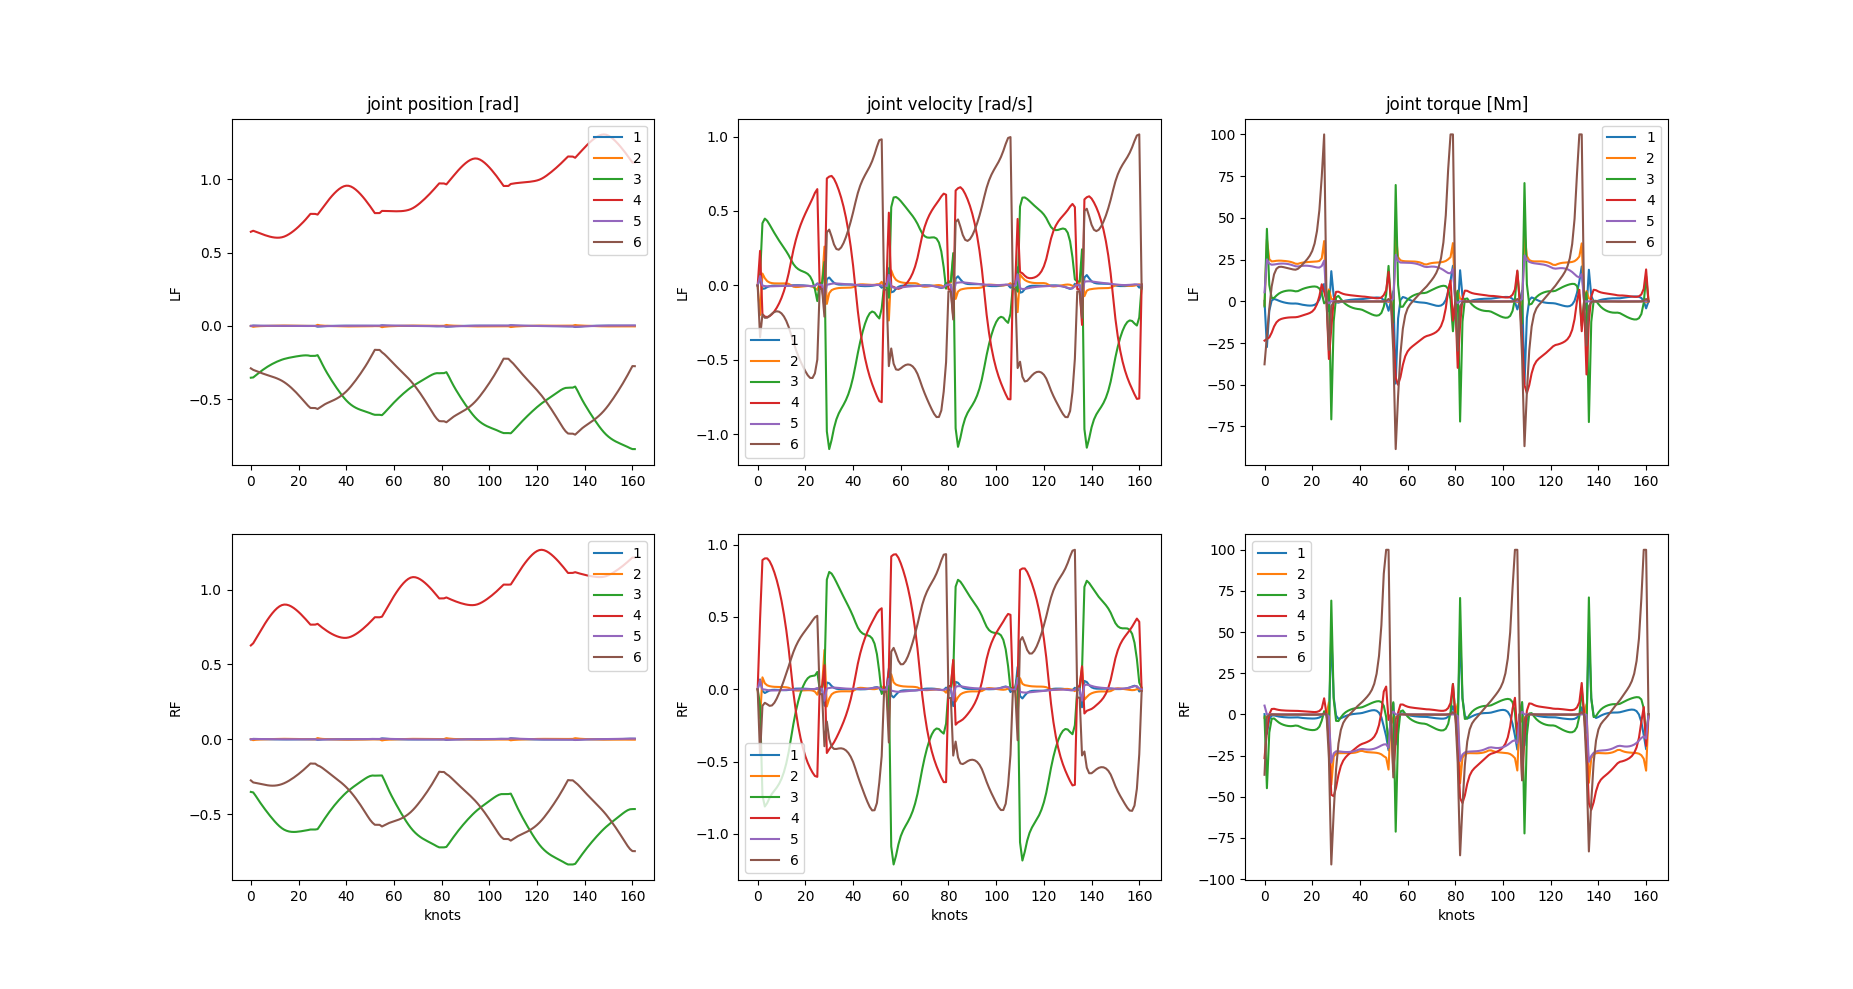
\includegraphics[width=1\linewidth]{Media/Crocoddyl/RH5/RH5GaitUbound50Percent_Solution.png}
  \caption{Solution for states and torques.}
\end{subfigure}
\begin{subfigure}{.8\textwidth}
  \centering
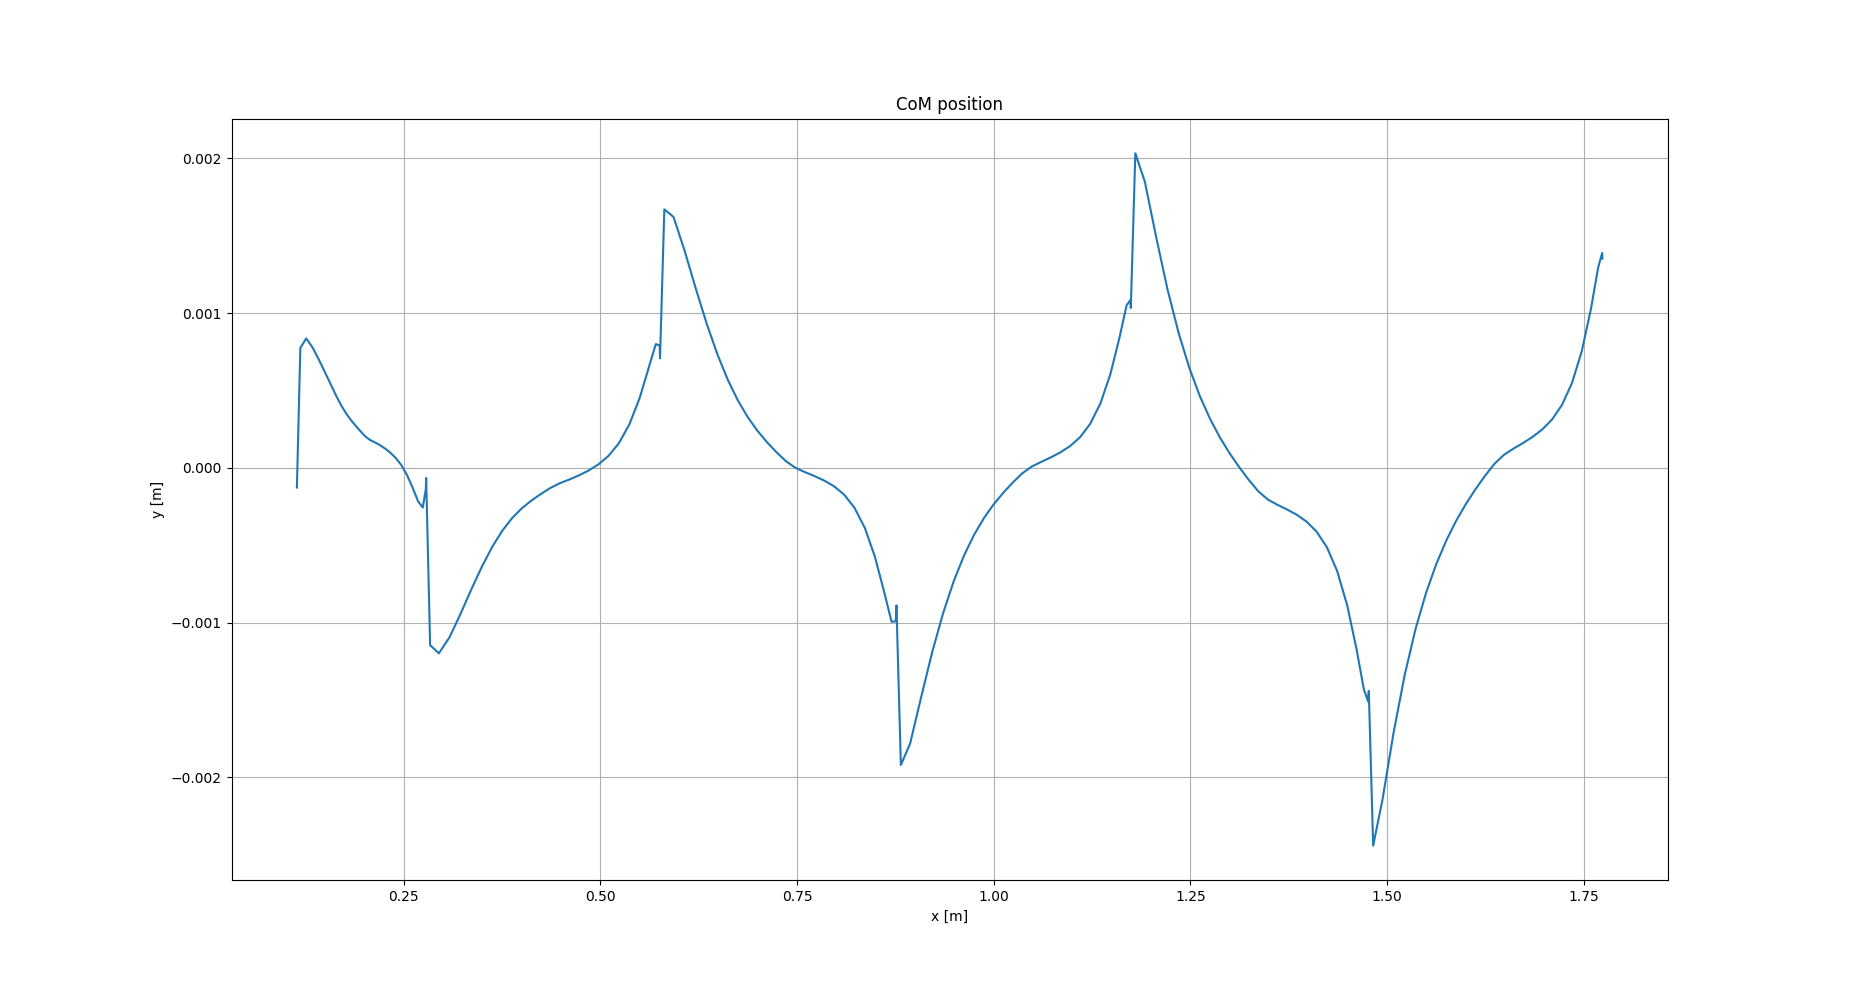
\includegraphics[width=1\linewidth]{Media/Crocoddyl/RH5/RH5GaitUbound50Percent_CoM.png}
\caption{CoM results.}
\end{subfigure}
\caption{Results for full gait with bounded input torques. To be even more restrictive, the available torques form the URDF have been reduced artificially by 50 percent. The effect becomes clear for e.g. the AnkleFT.}
\label{fig:rh5_constrain_torque}
\centering
\end{figure}

\subsection{Initial Pose Variants: Starting Near the Zero Configuration}
The full gait has been initialized according to the pose specifications from the RH5 DFKI smurf file. In this and the following section, two solutions for other initial poses are presented: One near the zero configuration and one at the zero configuration.

\begin{figure}[h!]
\centering
\begin{subfigure}{.8\textwidth}
  \centering
  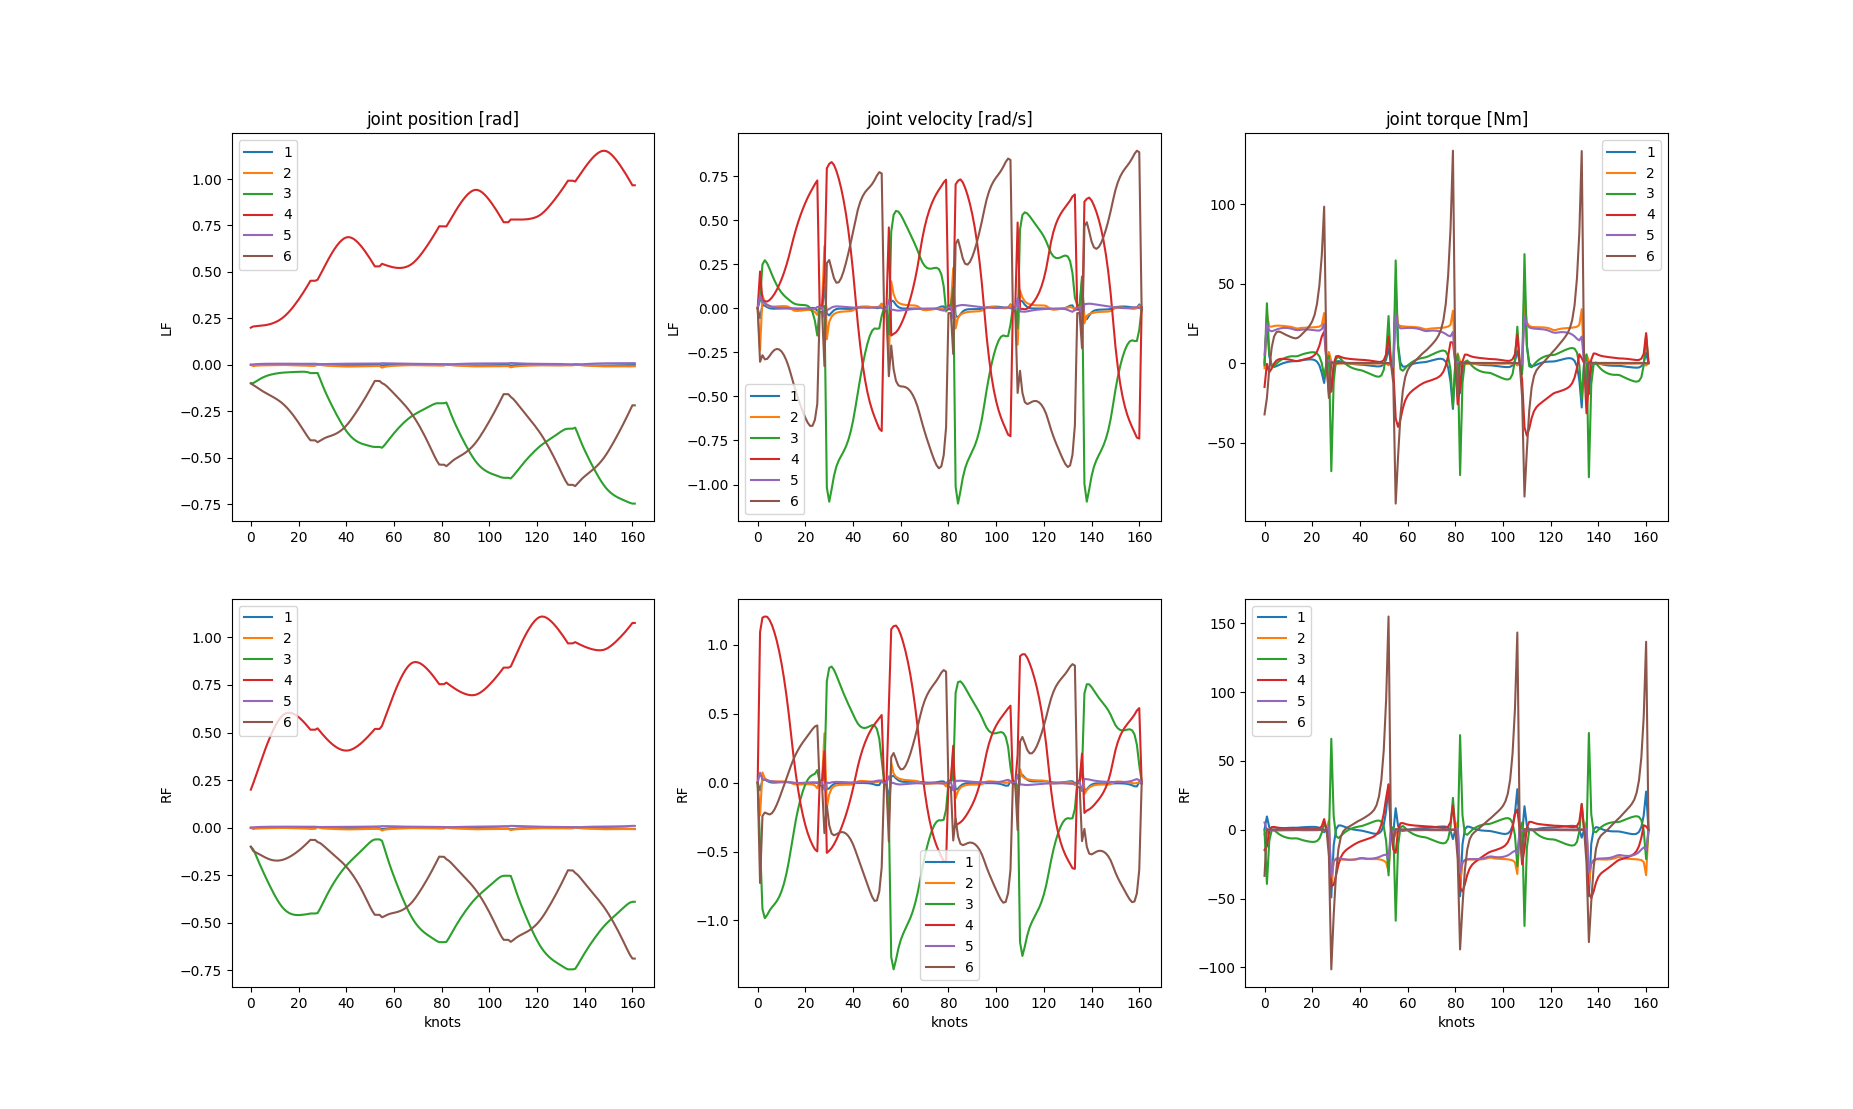
\includegraphics[width=1\linewidth]{Media/Crocoddyl/RH5/InitPoseVariants/RH5GaitInitNearZeroConfig_Solution.png}
  \caption{Solution for states and torques}.
\end{subfigure}
\begin{subfigure}{.8\textwidth}
  \centering
  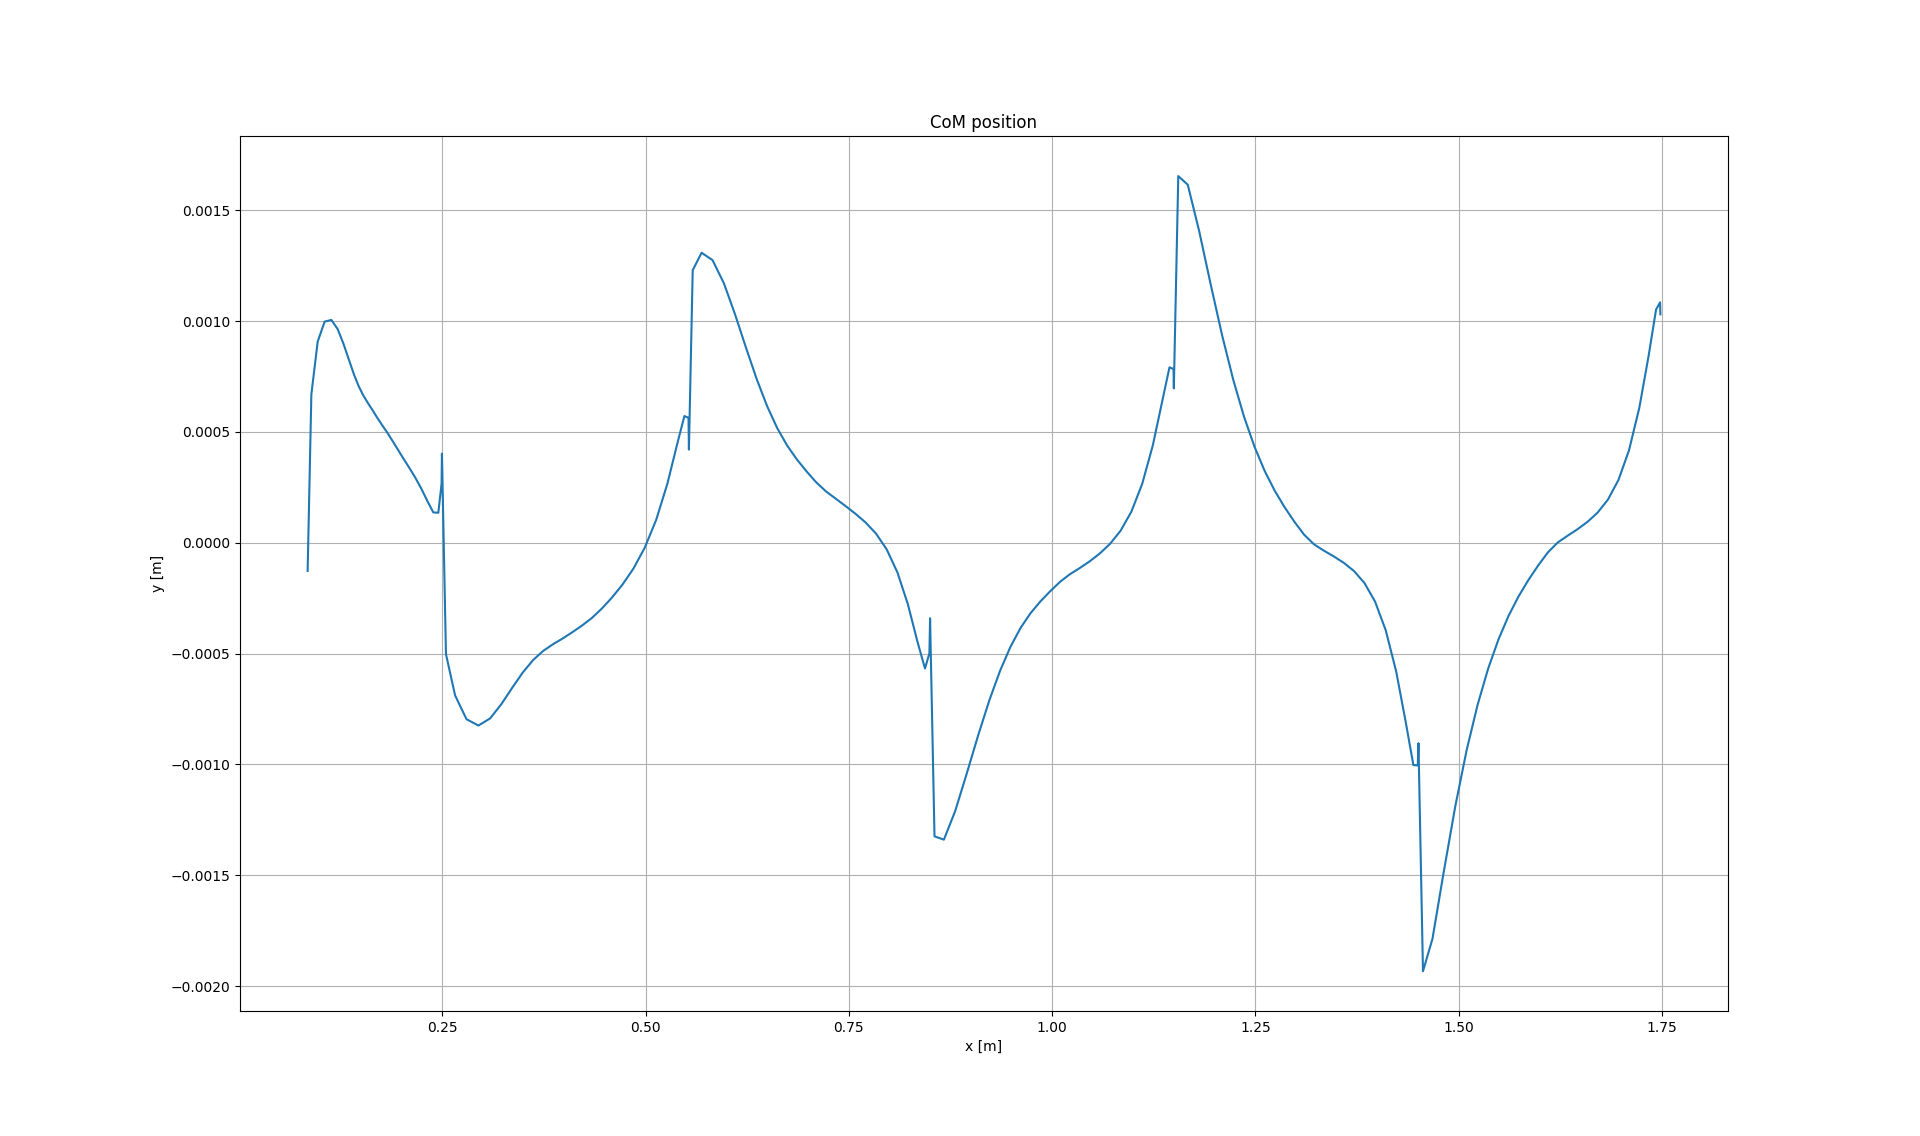
\includegraphics[width=1\linewidth]{Media/Crocoddyl/RH5/InitPoseVariants/RH5GaitInitNearZeroConfig_CoM.png}
\caption{CoM results.}
\end{subfigure}
\caption{Results for the full gait with initial pose \textbf{near} the zero configuration. q0=[0,0,-0.1,0.2,0,-0.1, 0,0,-0.1,0.2,0,-0.1] where  n=12 and represents the joint angles [rad] for the left and right leg.}
\label{fig:rh5_init_near_zero}
\centering
\end{figure}

\subsection{Initial Pose Variants: Starting At the Zero Configuration}
Initializing at the zero configuration turns out to be more critical. Sometimes the solver converges to a feasable solution (Figure \ref{fig:rh5_init_at_zero}), sometimes it does not find a proper solution (Figure \ref{fig:rh5_init_at_zero_failed_solver}).
\begin{figure}[h!]
\centering
\begin{subfigure}{.8\textwidth}
  \centering
  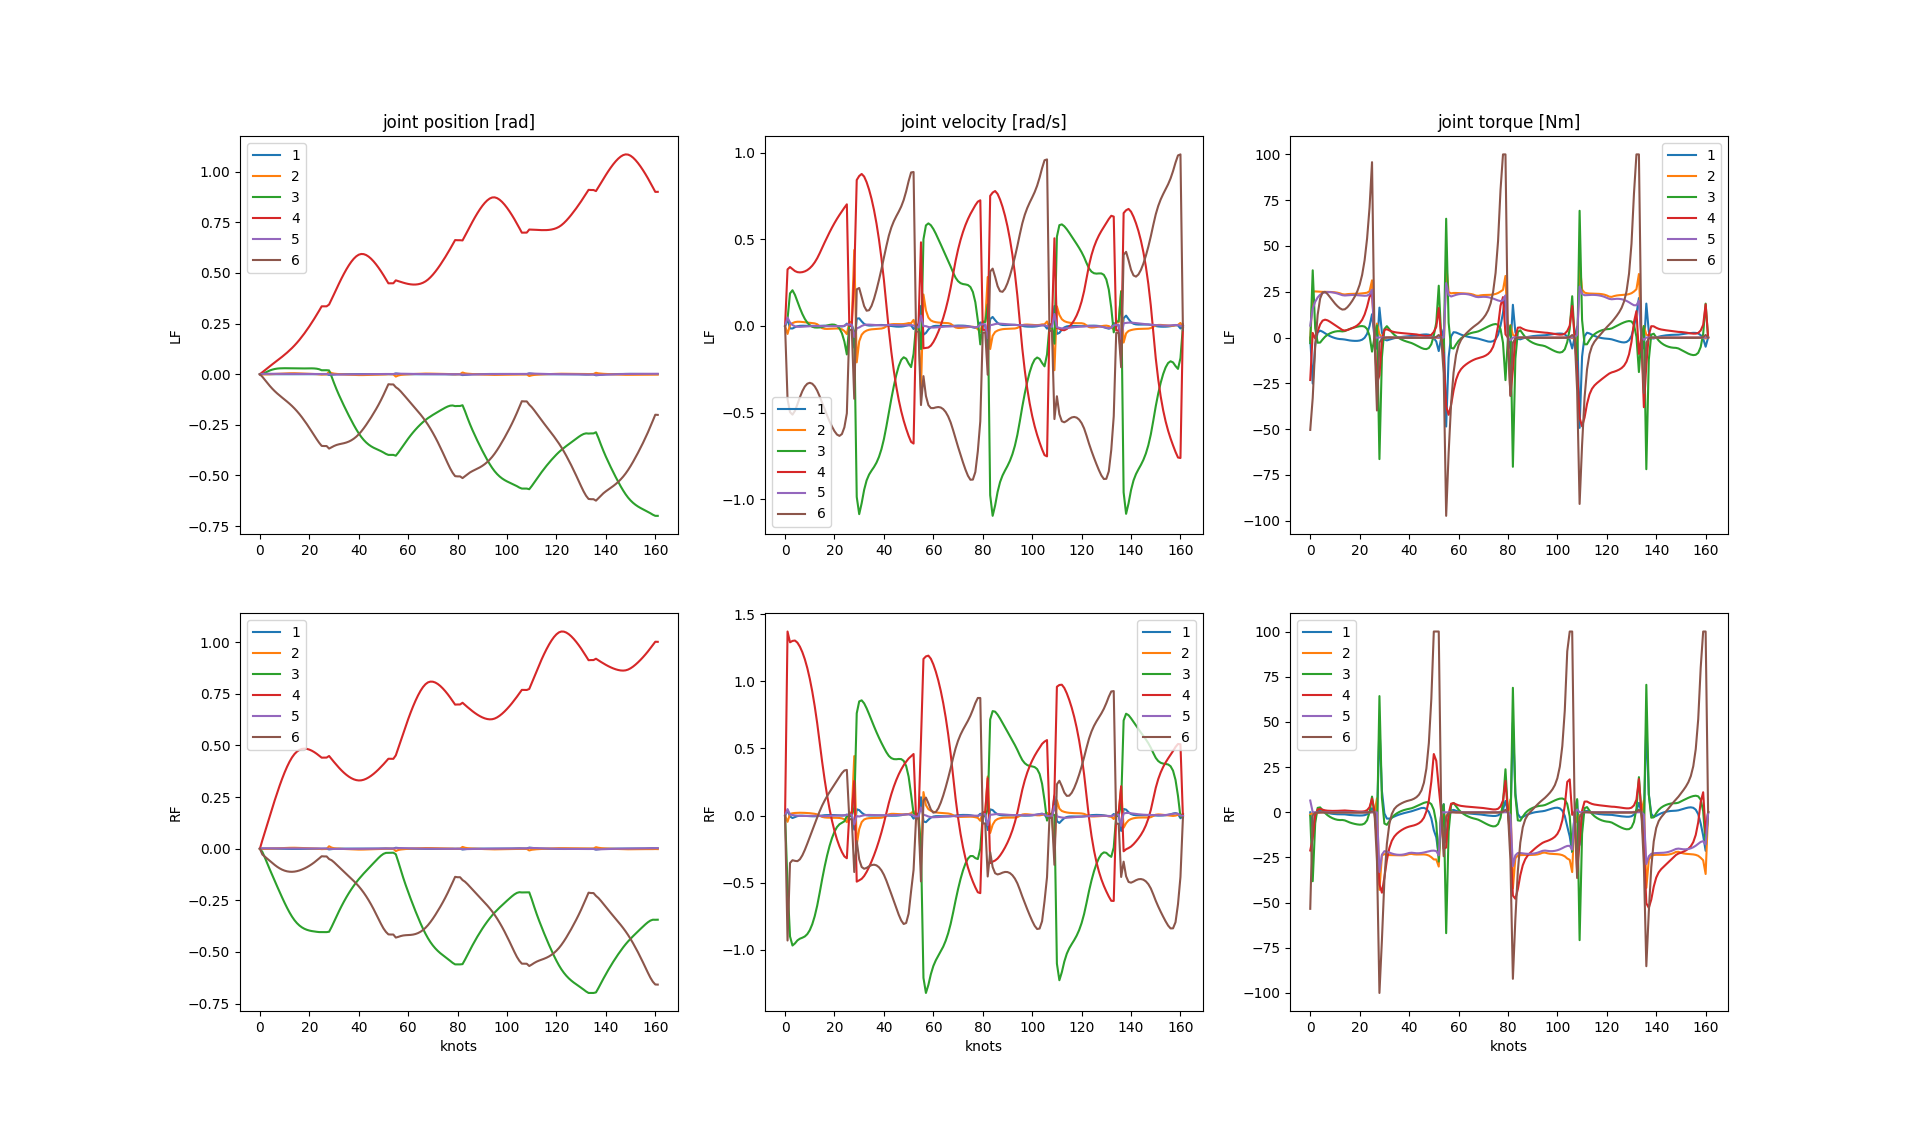
\includegraphics[width=1\linewidth]{Media/Crocoddyl/RH5/InitPoseVariants/RH5GaitInitZeroConfig_Solution.png}
  \caption{Solution for states and torques}.
\end{subfigure}
\begin{subfigure}{.8\textwidth}
  \centering
  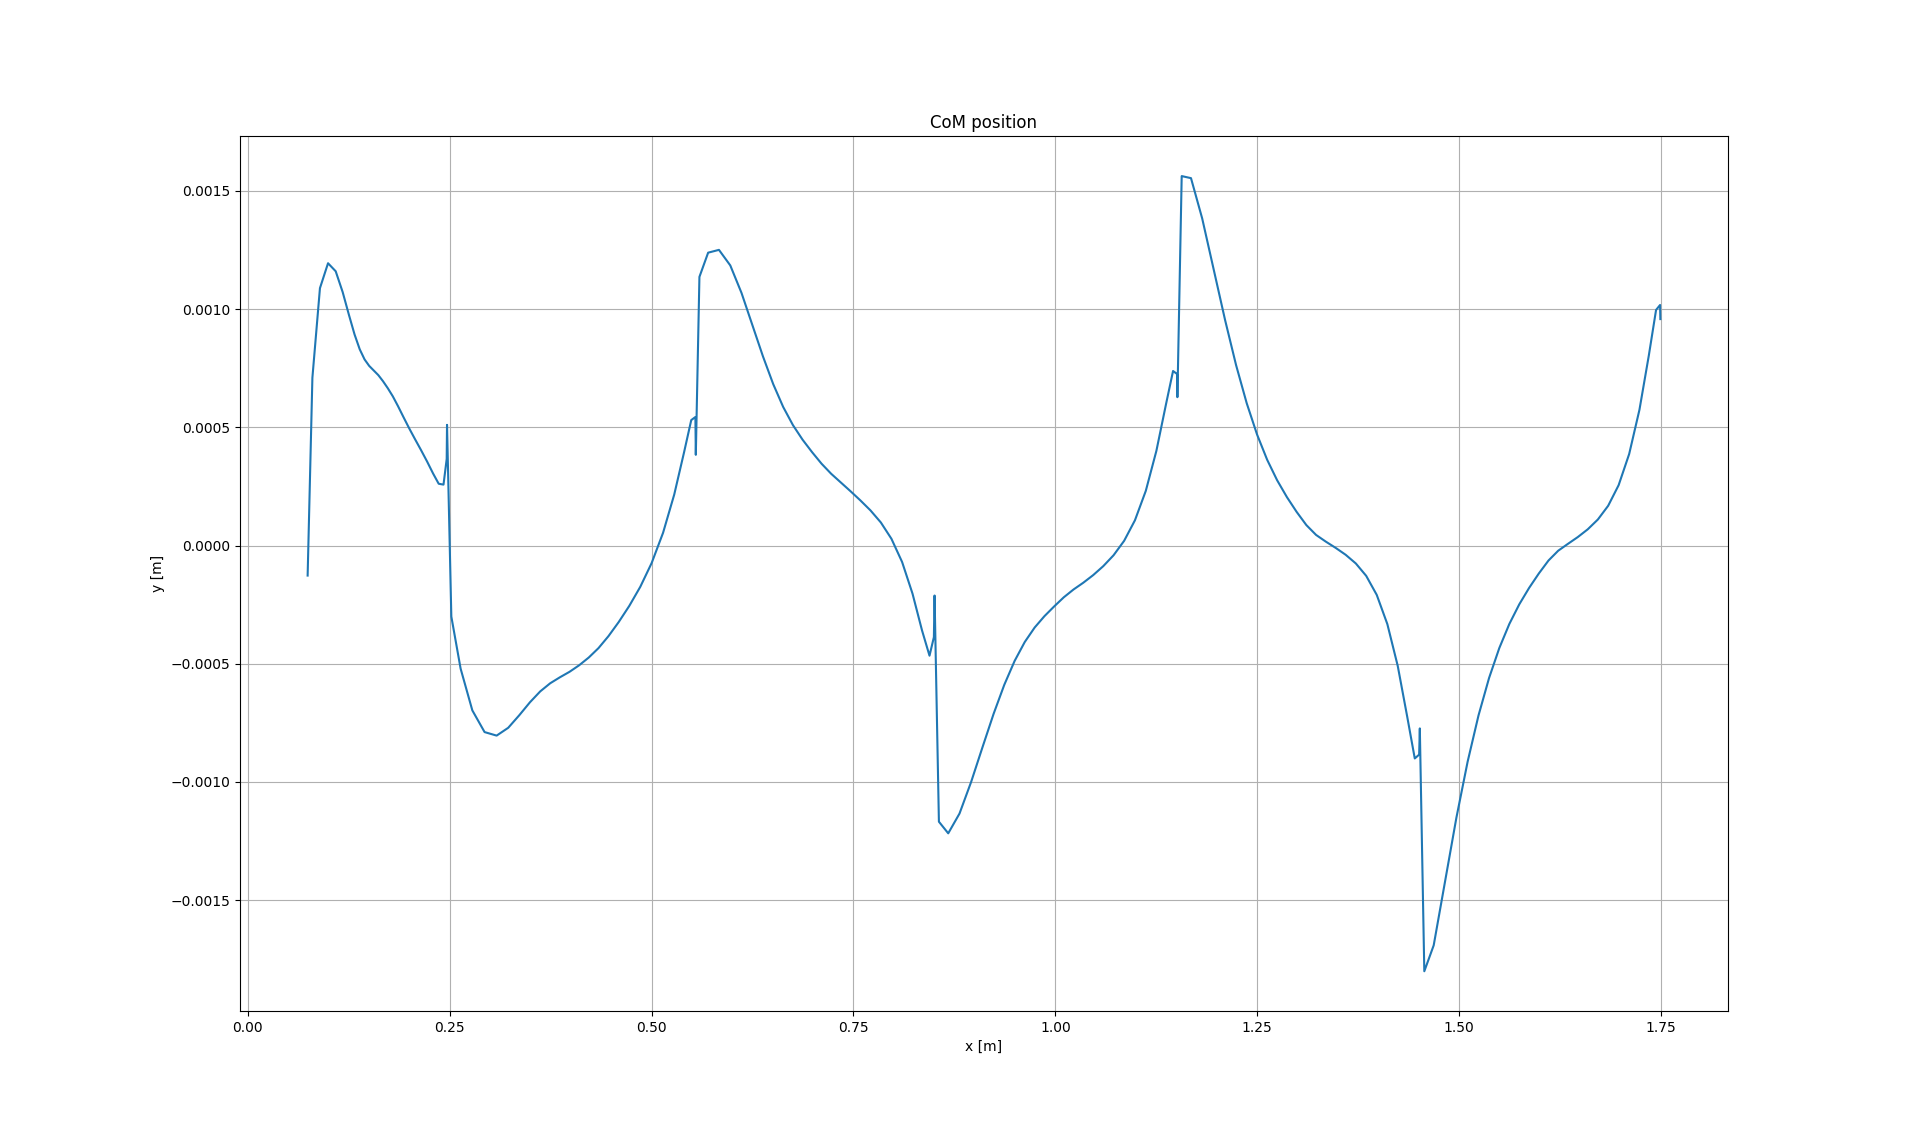
\includegraphics[width=1\linewidth]{Media/Crocoddyl/RH5/InitPoseVariants/RH5GaitInitZeroConfig_CoM.png}
\caption{CoM results.}
\end{subfigure}
\caption{Results for the full gait with initial pose \textbf{at} the zero configuration.}
\label{fig:rh5_init_at_zero}
\centering
\end{figure}

\begin{figure}[h!]
\centering
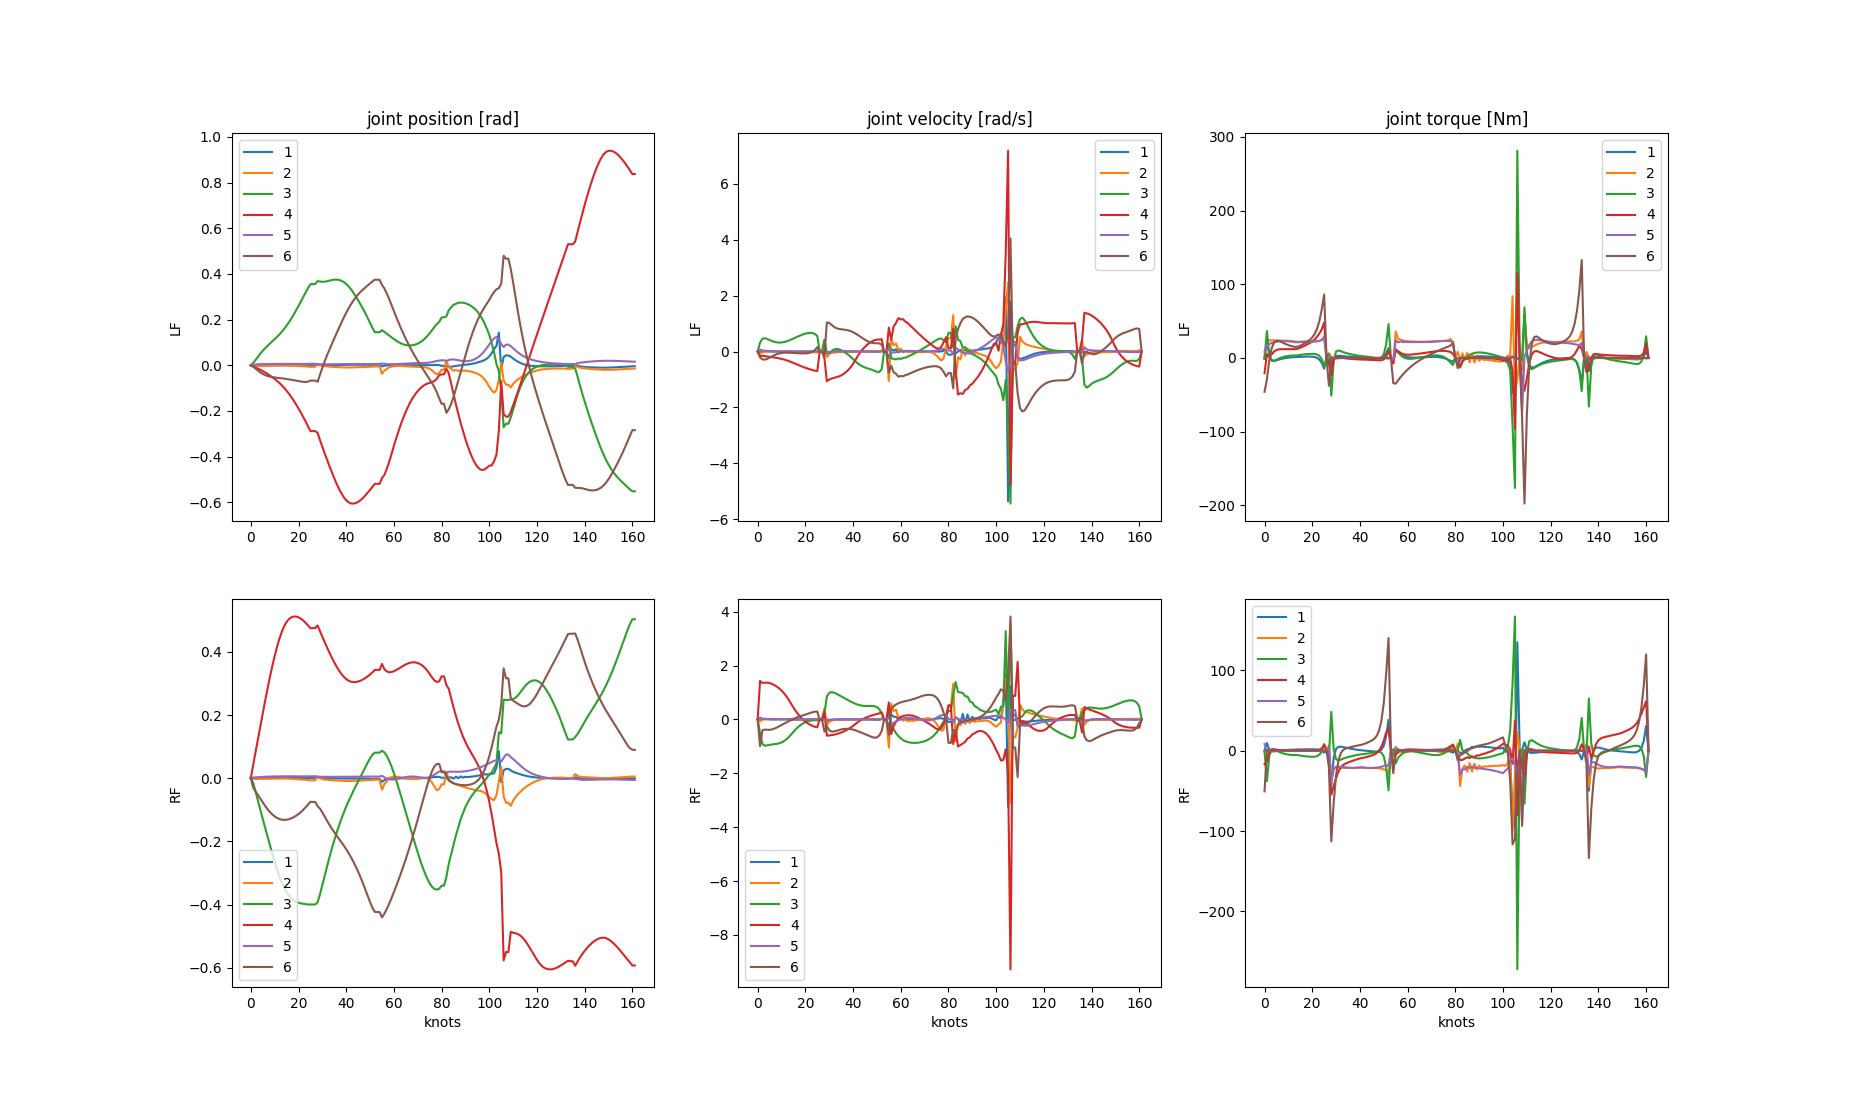
\includegraphics[width=1\linewidth]{Media/Crocoddyl/RH5/InitPoseVariants/RH5GaitInitZeroConfig_Solution_FailedSolver.png}
\caption{Another result for the full gait with initial pose \textbf{at} the zero configuration. The solution appears to be instable and would exceed the torque limits (see video).}
\label{fig:rh5_init_at_zero_failed_solver}
\end{figure}








 

\chapter{DRAKE - MIT CSAIL}
The second library we were interested in analyzing for its capabilites of generating bipedal walking patterns is Drake \cite{drake}. As it turned out, at the time of this work (spring 2020), Drake does not provide examples of legged locomotion anymore.  Because of limited time, such an example has not been implemented.

Consequently, this chapter starts with a brief introduction to Drake and then summarizes the work with some simple examples, especially passive dynamic walkers. The focus of this work has been shifted to enhance the results gained with the Crocoddyl library , as described in chapter \ref{chapter1}.  


\section{Introduction}
\subsection{Motivation}
Drake is a \textbf{C++ toolbox for}
\begin{itemize}
\item Analyzing the dynamics of robots
\item Building control systems for robots
\item Heavy emphasis on optimization-based design/analysis
\end{itemize}

Drake aims to \textbf{simulate} 
\begin{itemize}
\item Complex dynamics of robots (e.g. including friction, contact, aerodynamics etc.)
\item Emphasis on exposing the structure in the governing equations (sparsity, analytical gradients, polynomial structure, uncertainty etc.)
\item Making this information available for advanced planning, control, and analysis algorithms
\end{itemize}

Drake \textbf{provides}
\begin{itemize}
\item Python Interface
\item Implementation of state-of-the-art algorithms
\item Various examples
\end{itemize}

\subsection{Core Modules}
Drakes functionality is incorporated within several modules. This section gives a brief overview. 
\subsubsection{Modeling Dynamical Systems}
Drake uses a Simulink-inspired description of dynamical systems.

Includes basic building blocks (adders, integrators, delays, etc), physics models of mechanical systems, and a growing list of sensors, actuators, controllers, planners, estimators.
\subsubsection{Solving Mathematical Programs}
Drake's MathematicalProgram class is used to solve the mathematical optimization problem in the following form
$$min_{x} f(x) \quad s.t. x \in S$$
Depending on the formulation of the objective function $f$, and the structure of the constraint set $S$, Drake can solve the following categories of optimization problems
\begin{itemize}
\item Linear programming
\item Quadratic programming 
\item Nonlinear nonconvex programming
\item Semidefinite programming
\item Sum-of-squares programming
\item Mixed-integer programming
\end{itemize}
Drake \textbf{automatically} calls suitable solvers for each category of optimization problem.
\subsubsection{Multibody Kinematics and Dynamics}
\begin{itemize}
\item Drake's \textbf{constraint system} helps solve computational dynamics problems with algebraic constraints
\item Drake approximates real-world physical \textbf{contact} phenomena with a combination of geometric techniques and response models.
\end{itemize}

\section{How-To}
\subsection{Install}
Drake offers multiple ways of installation. This includes:
\begin{itemize}
\item Installation from Binaries
\item Installation from Source (using bazel)
\item Drake in Docker Containers
\end{itemize}
In this section some experiences for the installation from source and binaries are given. The choice mainly depends on if you want to use Drake via it's C++ or Python Interface. 
\subsubsection{Installation via Binaries}
Propably the easiest way to access the Drake functionalities is via \textbf{pydrake} (python bindings). In this case it should be sufficient to install the binaries of Drake and and access them from  a customized example directory, e.g. forked from the drake repo. 

For Ubuntu 18.04 the installation boils down to 
\begin{enumerate}
	\item Download and extract the latest version to your /opt 			directory:
	\begin{verbatim}
	curl -o drake.tar.gz https://drake-packages.csail.mit.edu/drake/		nightly/drake-latest-<platform>.tar.gz
	rm -rf /opt/drake
	tar -xvzf drake.tar.gz -C /opt
	\end{verbatim}
	\item Get the system dependencies:
	\begin{verbatim}
	/opt/drake/share/drake/setup/install_prereqs
	\end{verbatim}
	\item Add the python bindings to your PYTHONPATH environment 			variable:
	\begin{verbatim}
	export PYTHONPATH=/opt/drake/lib/python3.6/site-packages:$				{PYTHONPATH}
	\end{verbatim}
	\item Check if your installation was successful and that you can 	import pydrake:
	\begin{verbatim}
	python3 -c 'import pydrake; print(pydrake.__file__)'
	\end{verbatim}
\end{enumerate}
\subsubsection{Installation from Source Using Bazel}
If you instead prefer working directly on the \textbf{C++} examples or even want to contribute to the Drake library itself, an installation from source is recommended. 

Detailed instructions can be found here: \url{https://drake.mit.edu/from_source.html}.

Please note that the installation of Drake from source can take you \textbf{several hours}. 

\textbf{Issues during build process}

During installation from source I faced the following error message after a while:
\begin{verbatim}
Server terminated abruptly (error code: 14, error message: 'Socket closed'
\end{verbatim}
Maybe, this crash was caused by to less RAM (8GB). A workaround adapted from \url{https://stackoverflow.com/a/34399184} was to 
\begin{itemize}
\item Limit the number of parallel jobs and 
\item Limit the percentage of RAM Usage.
\end{itemize}
Finally, calling the build command with the following arguments was successfull:
\begin{verbatim}
CC=clang CXX=clang++ bazel build //... --ram_utilization_factor 30 --jobs=4
\end{verbatim}

\subsection{Run Python Examples}
Basically there are two kind of python examples provided:
\begin{itemize}
\item Encapsulated in a jupyter notebook (.jpnb): Interactively run the blocks
\item Pure python examples
\end{itemize}
The python examples can be found under the directory
\begin{verbatim}
/drake/bindings/pydrake/examples/multibody
\end{verbatim}
Within this directory, to run a \textbf{2D example} (using planar-scenegraph-visualizer):
\begin{verbatim}
python3 run_planar_scenegraph_visualizer.py
\end{verbatim}
If you instead want to run a \textbf{3D example} (using drake-visualizer):
In a first console open the visualizer from the binaries
\begin{verbatim}
/opt/drake/bin$ ./drake-visualizer
\end{verbatim}
Then, in a second console run (from your pydrake/examples/multibody directory again)
\begin{verbatim}
python3 cart_pole_passive_simulation.py
\end{verbatim}
to see a 3D visualization of the simulated dynamics of a cart-pole model.

\subsection{Additional Resources from MIT 6.832}\label{subsec:mit}
Additional to the examples provided within the drake, there is existing other useful material. The MITs Underactuated Robotics class \cite{mitx6.832web} offers a whole bunch of examples using pydrake. You can clone the repository with the course materials like this:
\begin{verbatim}
git clone https://github.com/RussTedrake/underactuated.git
sudo underactuated/scripts/setup/ubuntu/18.04/install_prereqs
export PYTHONPATH=`pwd`/underactuated:${PYTHONPATH}
\end{verbatim}


\section{Working with the Examples}
This section contains some applications of the Drake library within several examples. Herein, the focus lies on understanding the implementation, but additionally some insights about the system dynamics will be shown. 

Note that these examples are taken from Drake, but from the \href{http://underactuated.csail.mit.edu/underactuated.html}{MIT Underactuated Robotics class}. See section \ref{subsec:mit} for details on how to get the examples. The videos can all be found under \url{https://github.com/julesser/oc-frameworks/tree/master/OCFrameworks/Media/Drake}. 

\subsection{Cart-Pole}
One classic example of a simple underactuated system is the famous cart-pole model. The system has 2DOF $\theta, x$, where only the horizontal position $x$ is acutated. 
For further details on the system visit \url{http://underactuated.csail.mit.edu/acrobot.html#cart_pole}.
\subsubsection{Balancing around the upright using LQR}
The \href{http://underactuated.csail.mit.edu/lqr.html}{Linear Quadratic Regulator (LQR)} solves linear time-invariant system where the cost is described by a quadratic function.
An exemplary task can be to stabilize the uprgith position of the pendulum from initial conditions.

\subsubsection{Trajectory Optimization using Direct Collocation}
From a methodology point of view, this example is interesting for our research and therefore will be explained in a bit more detail. The resulting dynamic up-swinging and and stabilization can best be seen in the \href{https://raw.githubusercontent.com/julesser/oc-frameworks/master/OCFrameworks/Media/Drake/ExSimple/CartpoleTrajOptDirCol.mp4}{videos}, while the optimal force solution presented in Figure \ref{fig:cart-pole}.
\begin{enumerate}
\item Load and build the dynamic model (\textit{plant+context})
\begin{verbatim}
plant = MultibodyPlant(time_step=0.0)
scene_graph = SceneGraph()
plant.RegisterAsSourceForSceneGraph(scene_graph)
file_name = FindResource("models/cartpole.urdf")
Parser(plant).AddModelFromFile(file_name)
plant.Finalize()
context = plant.CreateDefaultContext()
\end{verbatim}
\item Setup the optimization problem with discrete, uniform time steps (i.e. knots)
\begin{verbatim}
dircol = DirectCollocation(
    plant,
    context,
    num_time_samples=21,
    minimum_timestep=0.1,
    maximum_timestep=0.4,
    input_port_index=plant.get_actuation_input_port().get_index())
dircol.AddEqualTimeIntervalsConstraints()
\end{verbatim}
\item Specify the initial and terminal state via constraints
\begin{verbatim}
initial_state = (0., 0., 0., 0.)
dircol.AddLinearConstraint(dircol.initial_state() == initial_state)
final_state = (0., math.pi, 0., 0.)
dircol.AddLinearConstraint(dircol.final_state() == final_state)
\end{verbatim}
\item For each running knot, penalize actuator effort. For the terminal state, penalize the total time consumped.
\begin{verbatim}
R = 10  # Cost on input "effort".
u = dircol.input()
dircol.AddRunningCost(R * u[0]**2)
dircol.AddFinalCost(dircol.time())
\end{verbatim}
\item Generate a piecewise-polynomial function and use it as initial guess
\begin{verbatim}
initial_x_trajectory = PiecewisePolynomial.FirstOrderHold(
    [0., 4.], np.column_stack((initial_state, final_state)))  
dircol.SetInitialTrajectory(PiecewisePolynomial(), initial_x_trajectory)
\end{verbatim}
\item Solve the trajectory optimizaton problem
\begin{verbatim}
result = Solve(dircol)
\end{verbatim}
\end{enumerate}

\begin{figure}[h!]
\centering
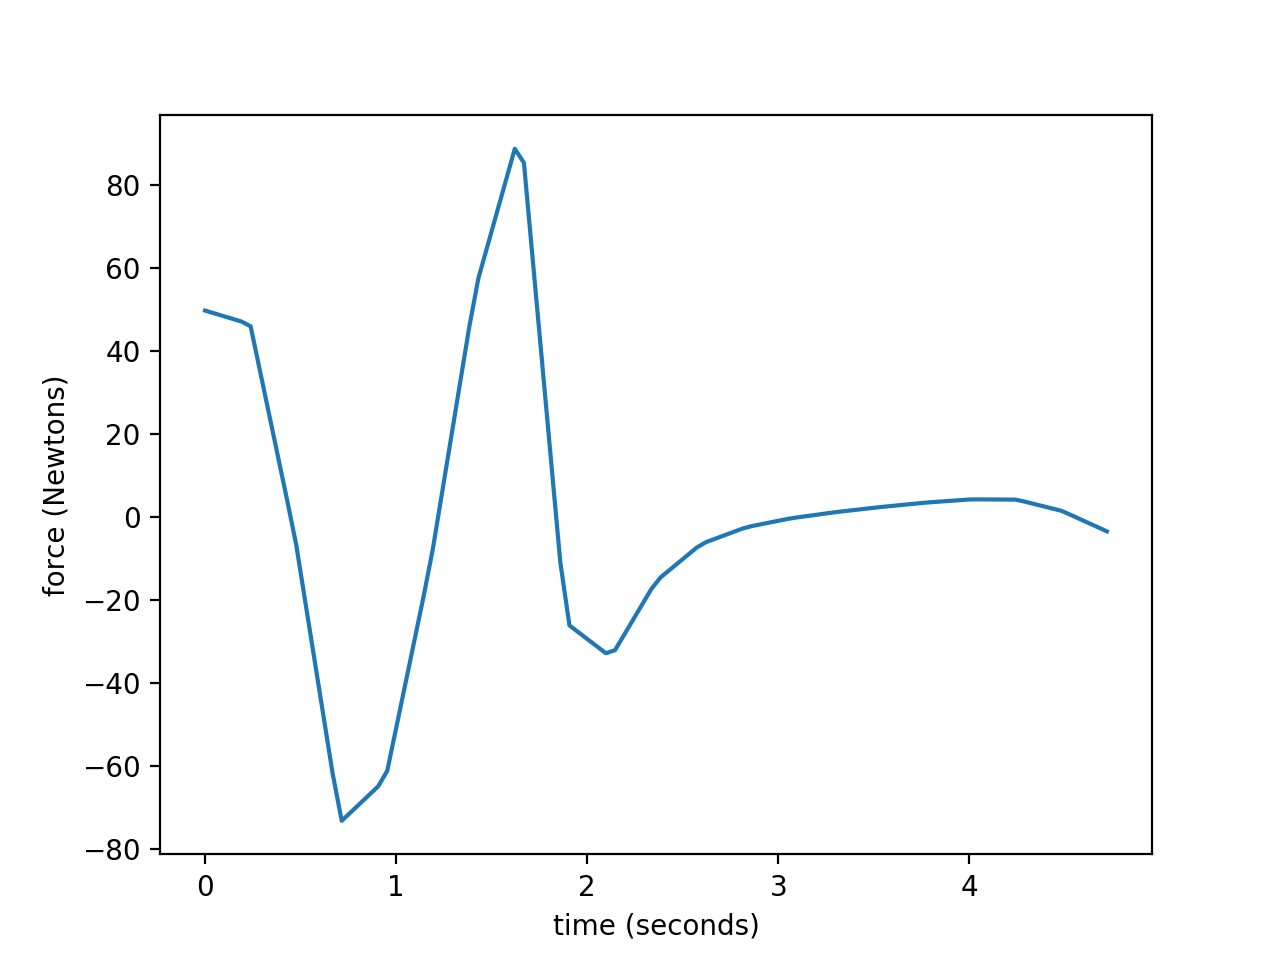
\includegraphics[width=.7\linewidth]{Media/Drake/ExSimple/CartPoleTrajOptDirCol_Solution.png}
\caption{Resulting optimal horizontal force from trajectory optimization of the up-swining and stabilization for the cart-pole.}
\label{fig:cart-pole}
\end{figure}

\subsection{Passive Dynamic Walkers}
Although there currently are no highly-articulated robots found in the Drake examples, it does provide some classic examples of simplified locomotion models. 

\subsubsection{Rimless Wheel}
Simulating the simple dynamics of the rimless wheel model rolling down a declining slope, an continous limit cycle emerges (see Figure \ref{fig:rimlessWheel}).
\begin{figure}[h!]
\centering
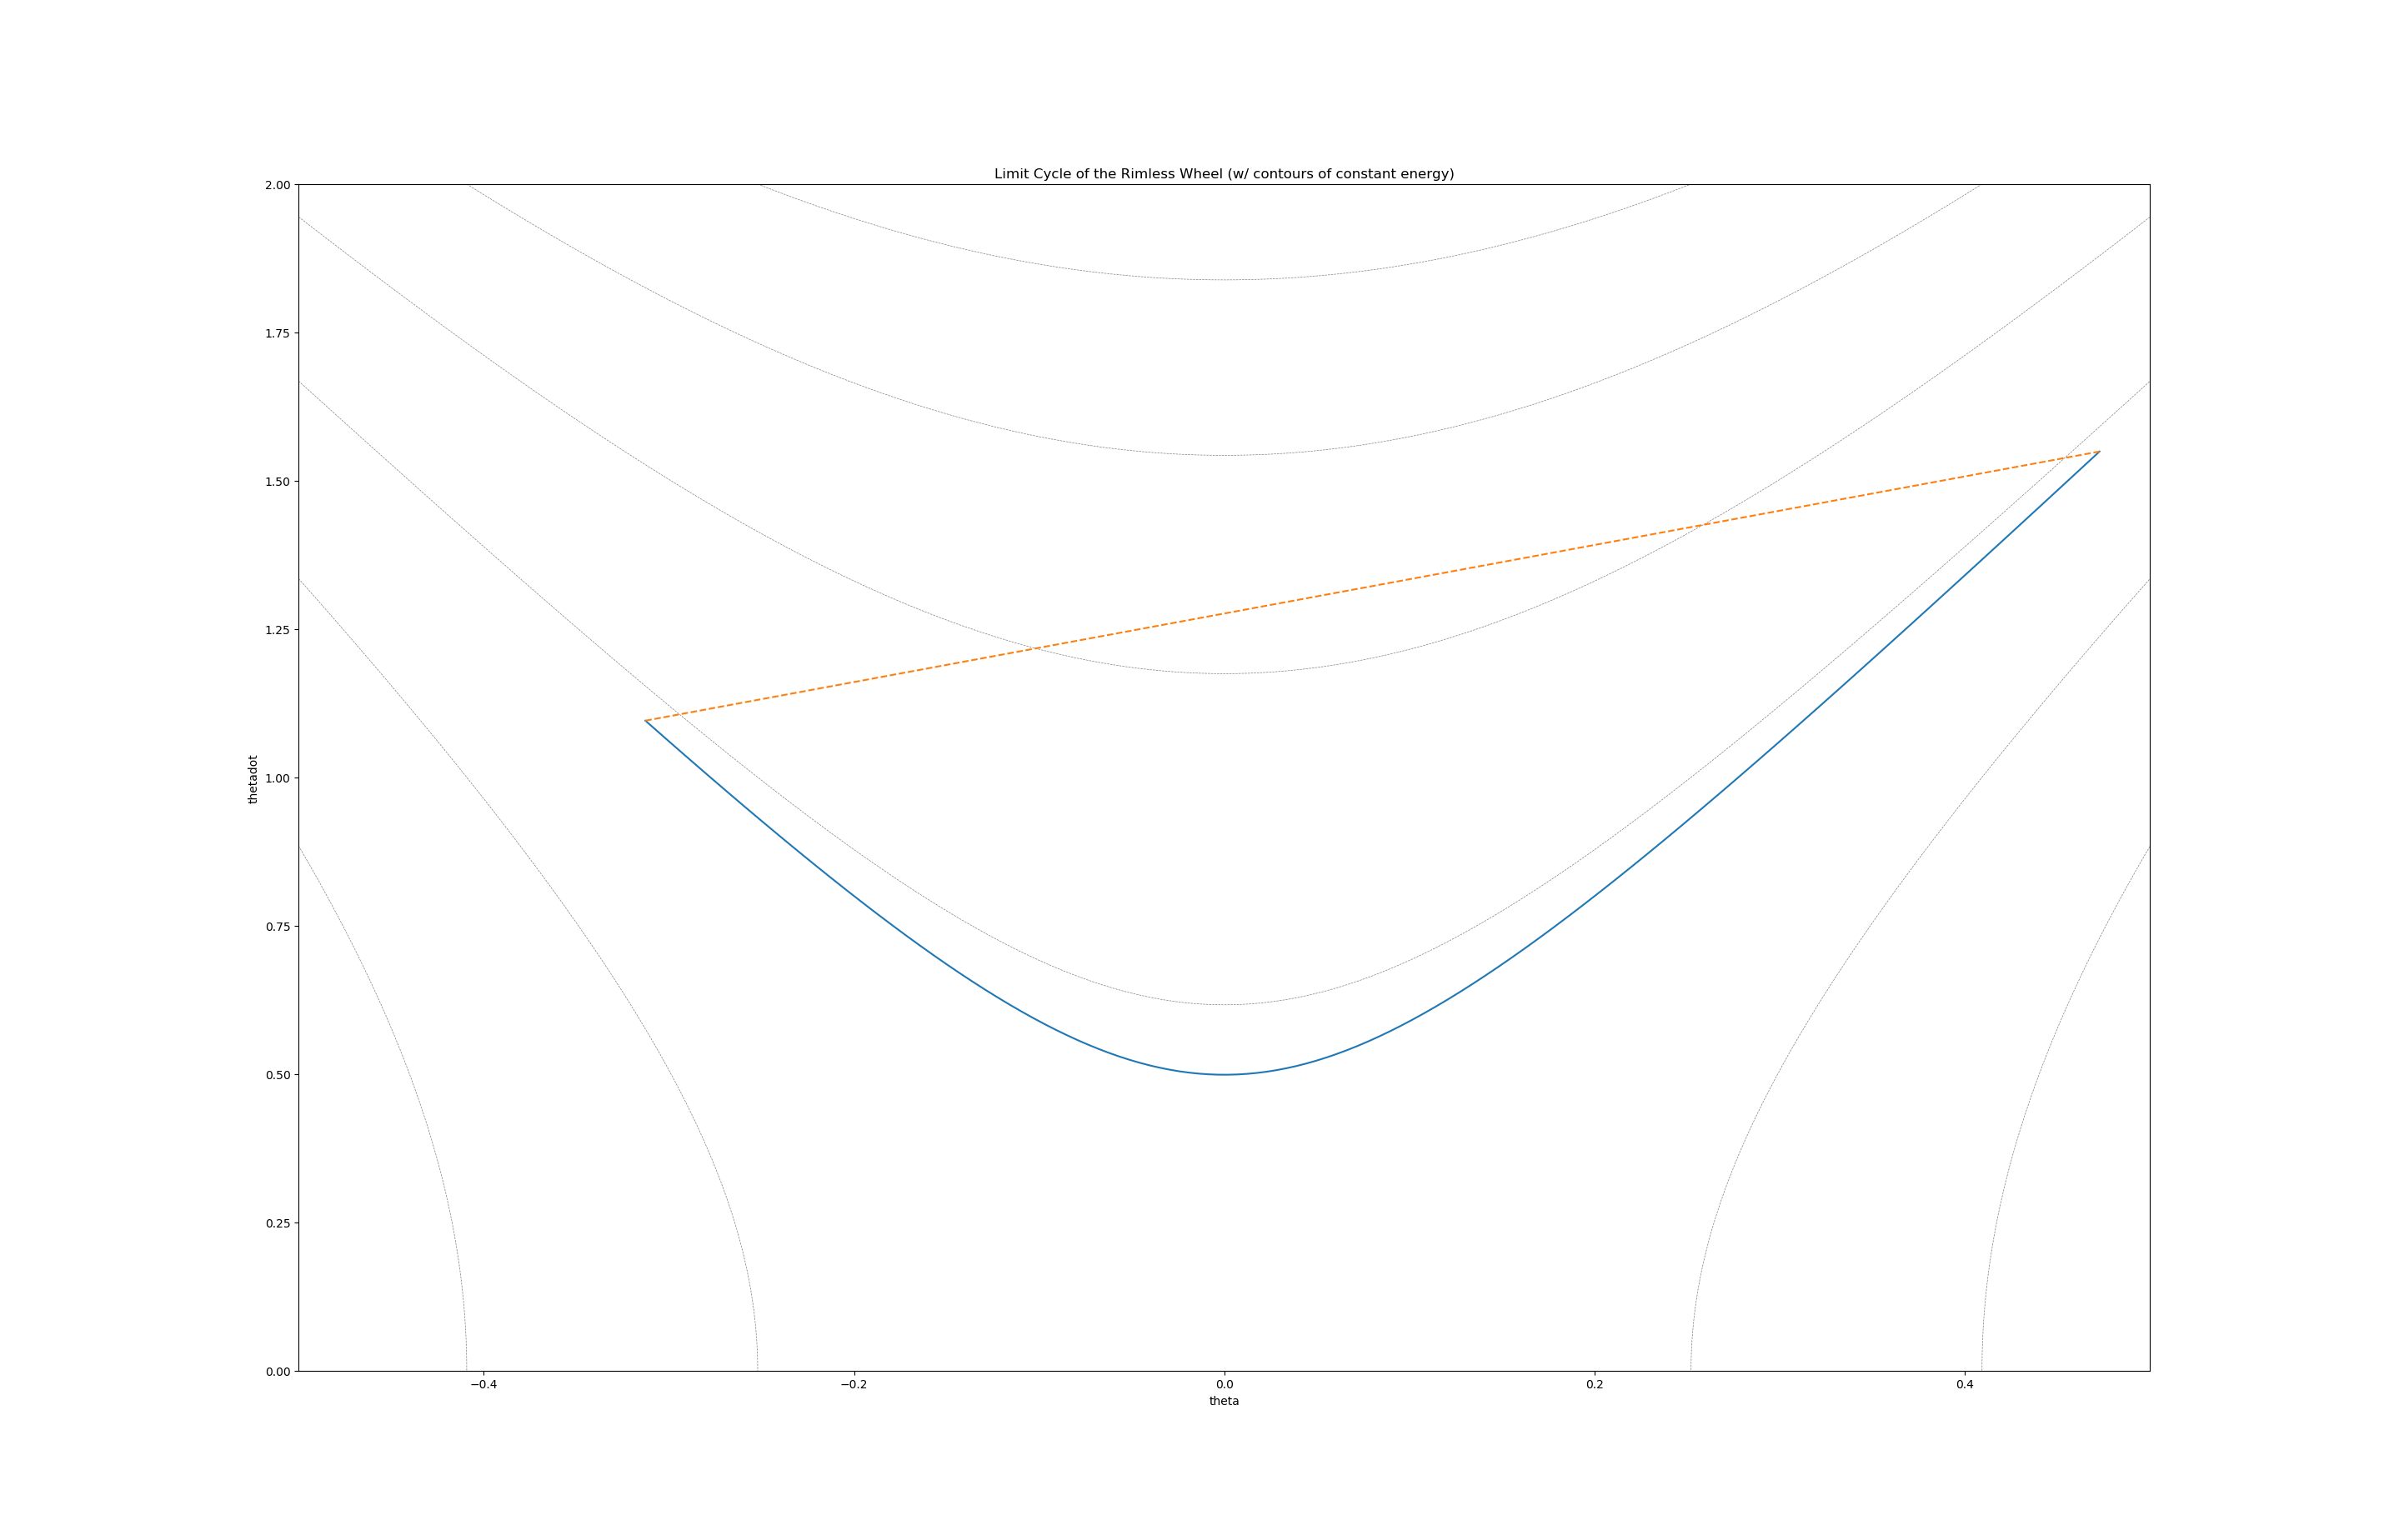
\includegraphics[width=1\linewidth]{Media/Drake/ExSimpleWalking/RimlessWheelDirCol_LimitCycle.png}
\caption{Results for an energy-optimal limit cycle for the rimless wheel using direct collocation trajectory optimization.}
\label{fig:rimlessWheel}
\end{figure}

\subsubsection{Compass Gait}
The compass gait is a simple bipedal walking model containing two links and three pointmasses. For further details on the system visit \url{http://underactuated.csail.mit.edu/simple_legs.html#section2}. 

Simulating the system dynamics for a declining slope results in periodic motions (see Figure \ref{fig:compassGait}).
\begin{figure}[h!]
\centering
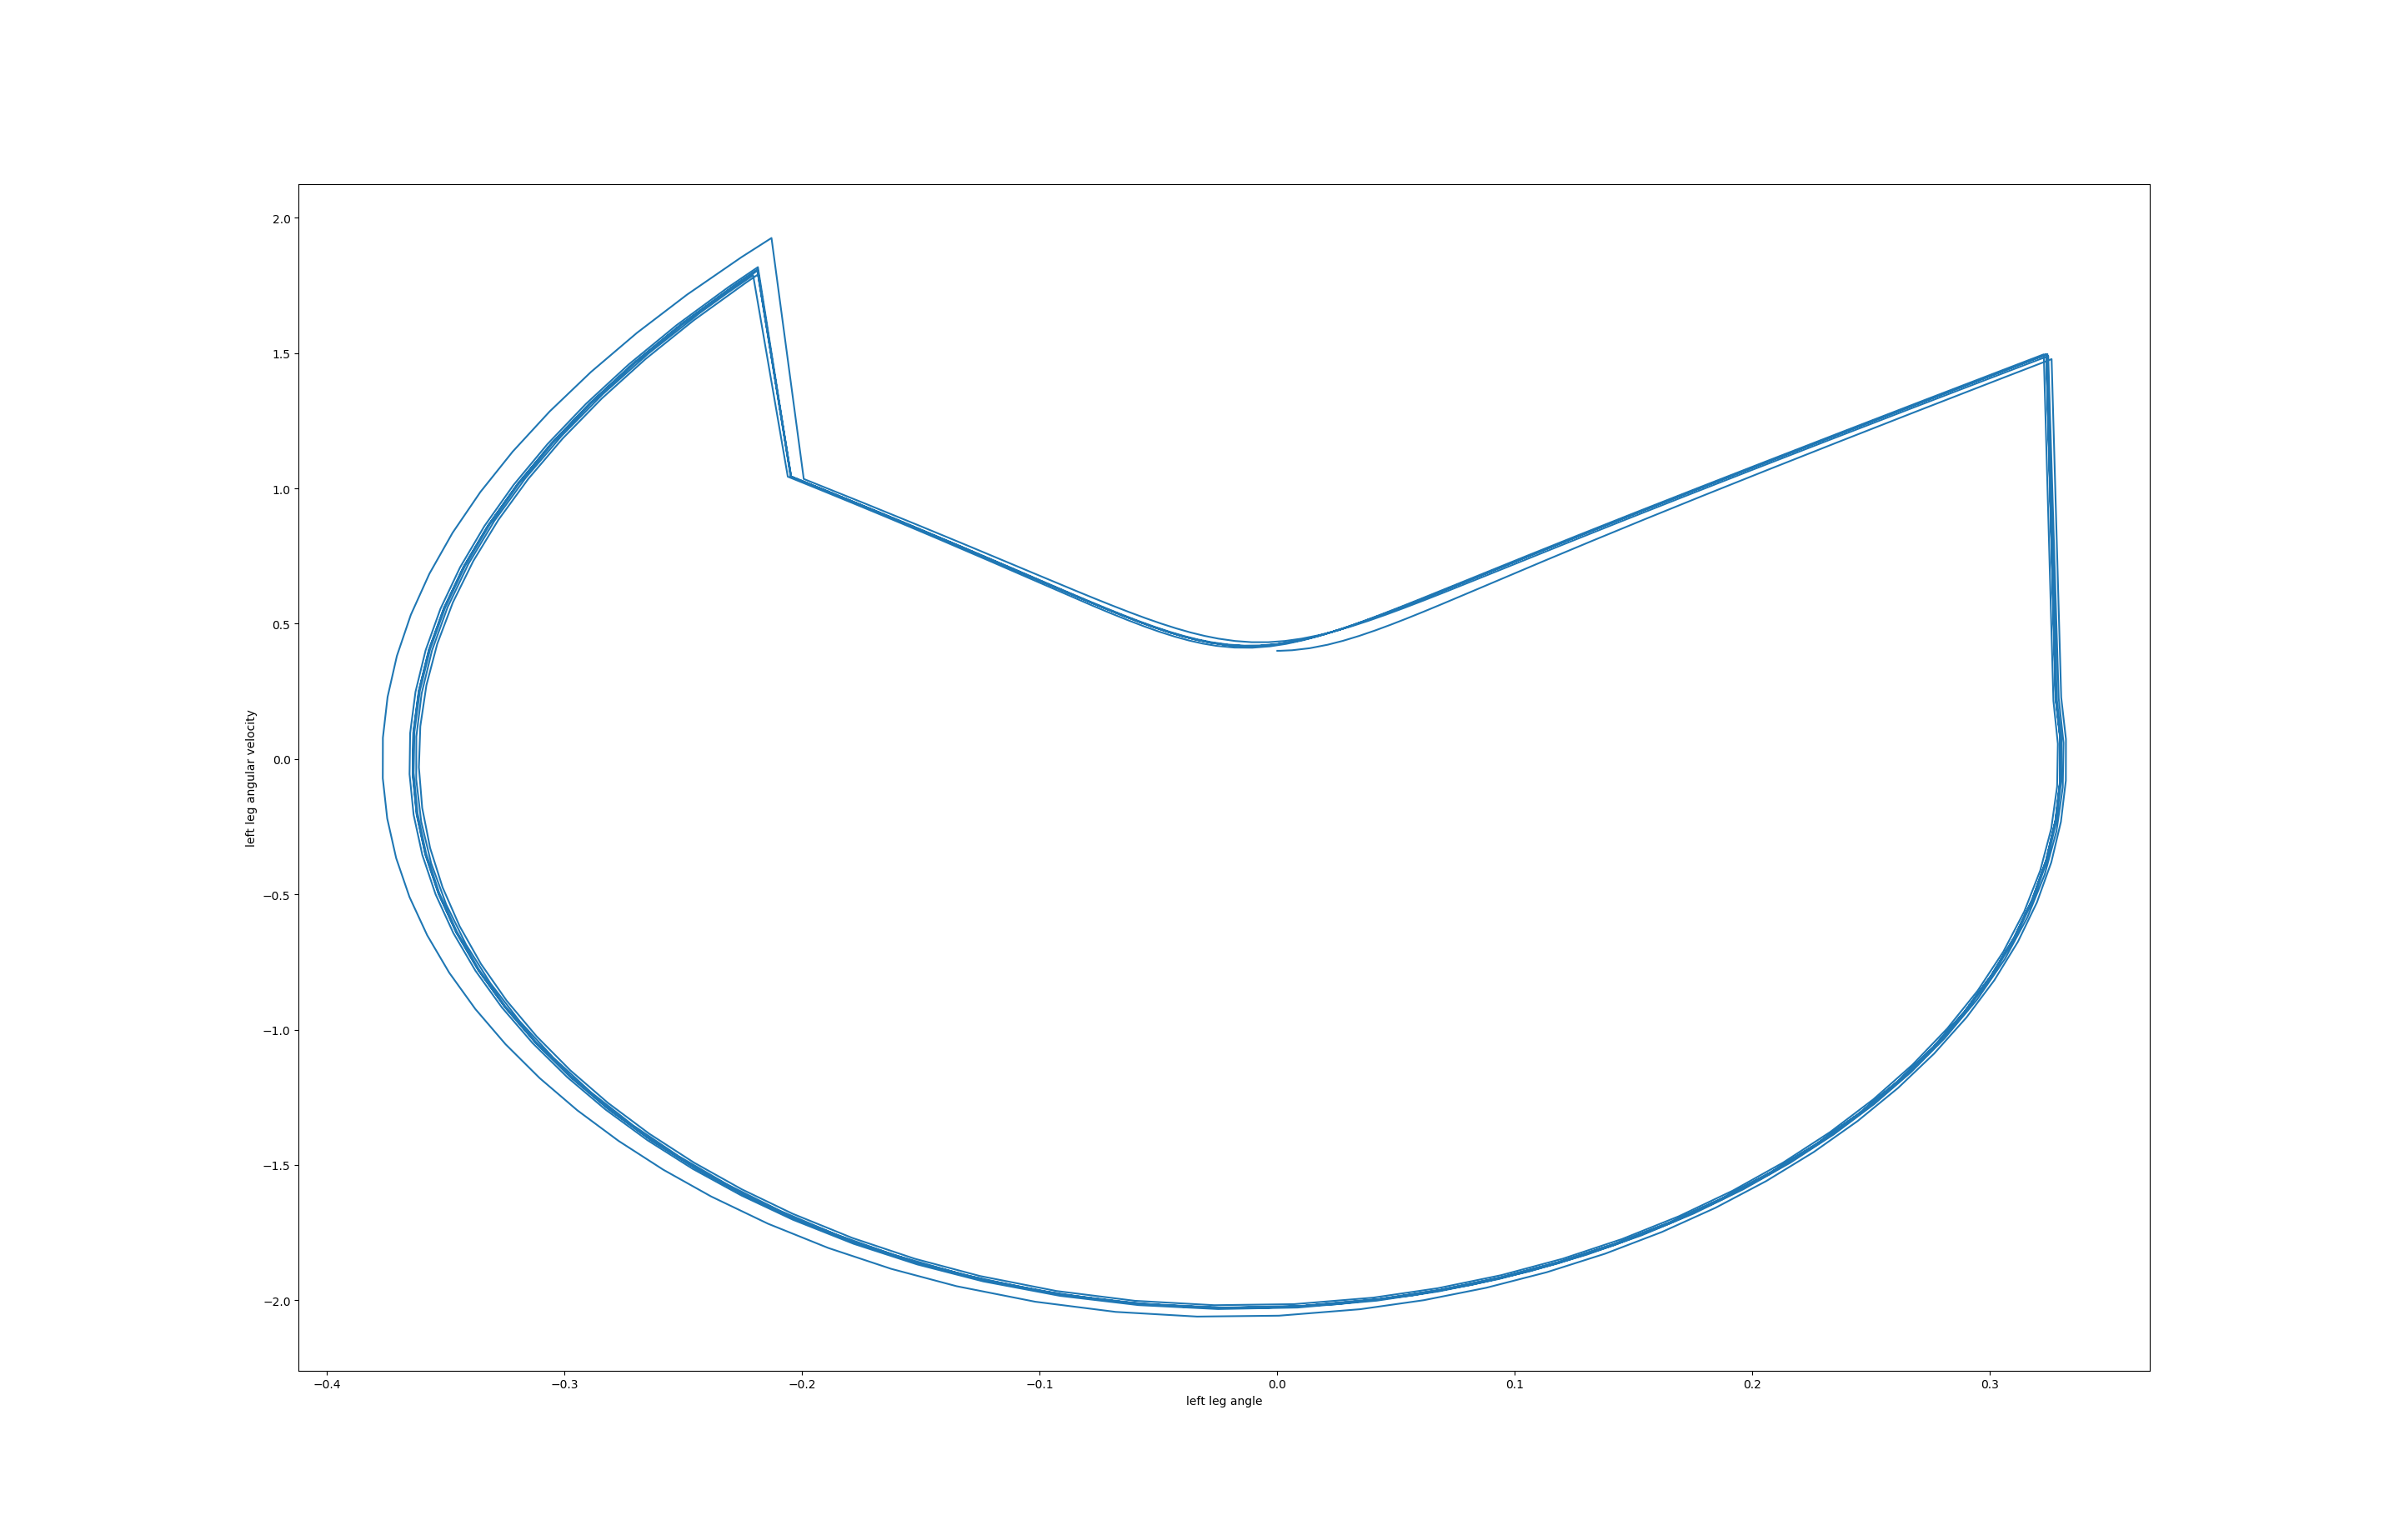
\includegraphics[width=1\linewidth]{Media/Drake/ExSimpleWalking/CompassGait_PhasePlot.png}
\caption{Resulting phase plot of the compass gait reveals periodic orbits.}
\label{fig:compassGait}
\end{figure}




\chapter{COMPARISON}
This chapter offers a brief comparison of both frameworks in terms of generality, usability and bipedal walking capabilities. This comparison is from a very practical point of view and may be biased since the author investigated Crocoddyl more strongly than Drake.  Furthermore, this work is context-specific to generating optimal trajectories for a simple bipedal walking pattern.

 
\section{Generality vs Specificity}
Both frameworks differ considerably in the variety of problems that they are trying to takle and the amount of implemented functionalities. 

For solving optimal control problems, each of the frameworks follows its own path.

\subsubsection{Overall Scope}

Drake to a certain extend is a 'All in One' library since it contains modules for solving multibody dynamics, mathematical programs as well as a whole bunch of tools for modeling and analyzing systems to gain a deeper understanding of the underlying dynamics.
On the opposite, Crocoddyl is designed for a very specific range of problems, namely to solve optimization problems for robots with multiple point-contacts. It depends on the Gepetto-Viewer for visualizing and the Pinnoccio library for kinematics formulation and dynamics calculations.

\subsubsection{Optimal Control Solvers}

Also the way the optimization problems are solved differ quite strong. Whereas Drake offers a wide range of available solvers, Crocoddyls solvers list in comparison is rather small and solely based on versions of the Differential Dynamic Programming (DDP) algorithm. 

\subsubsection{Formulation of Trajectory Optimization}

Finally, the way of \href{http://underactuated.csail.mit.edu/trajopt.html#section2}{discretising the continous time-problem} for the trajectory optimization methods differs. Crocoddyl on the one hand focuses on shooting methods, while Drake on the other hand utilizes direct transcription/collocation.


\section{Usability}
In general, the author considers Drake as well as Crocoddyl to be quite user-friendly, but Drake stands out with its excellent code documentation.

\subsubsection{Python Bindings}
The main reason for this assessment propably is the provision of python bindings within both libraries, which allows for rapid prototyping of examples. 

\subsubsection{Installation}
To this end, the installation procedure could be simplified a lot since it was sufficient to install the binaries under /opt and use a cloned version of the examples directory. Following this approach, the Drake binaries can be installed as usual, while Crocoddyl utilizes the \textit{robotpkg} manager.

\subsubsection{Code Documentation}
Drake offers a beautiful \href{https://drake.mit.edu/doxygen_cxx/index.html}{descripiton} of it's C++ API that also holds for most of the functionalities within pydrake. Crocoddyl on the other hand provides only a very sparse documentation, e.g. on solver functionalities or implemented contact models. 

\subsubsection{Getting Started}
What Crocoddyl lacks in code documentation is definitely made up for by an excellent collection of beginner-friendly tutorials! Drake also comes along with some beginner tutorials, but in the authors opinion the tend to be more abstract.

\subsubsection{Example Functionalities}
Also in the example domain Croccodyl can shine. Whereas Drake  solely offers examples related containing simple systems, Crocoddyl provides the user with readily accessible examples of complex legged robots (e.g. quadrupeds, humanoids) performing challenging tasks (e.g. walking, jumping).


\section{Bipedal Walking Capabilities}\label{sec:BipedWalkCapabilities}
The example of bipedal walking provided by the Crocoddyl library served as a comfortable starting point for integrating and testing the RH5  robot (see section \ref{sec:resultsRH5} for the results).

On the contrary, Drake currently does not offer this luxury. The goal of this section is to estimate the effort necessary to produce equivalent bipedal walking results within the Drake library that already have been achieved within Crocoddyl.

% TODO: Add estimation of effort & possible issues producing bipedal walking with Drake 

\subsection{RH5 Example in Drake: Key Components}
In the following, the key steps towards a functional bipedal walking example shall be determined and crosschecked with the functionalities Drake provides. 

\subsubsection{High-Level Formulation:}
\begin{enumerate}
\item Build and visualize the robot via a URDF-based description
\item Implement basic locomotion logic (Double support, foot step)
\item Generate reference trajectory, i.e. initial guess
\item Formulate an optimization problem with discrete time-steps
\begin{itemize}
\item Constrain the problem (e.g. bounded torques) 
\item Time-step specific costs 
\item Time-step specific point-contacts 
\item Model impulse dynamics
\end{itemize}
\item Solve the problem with sophisticated method
\end{enumerate}
\subsubsection{Step 1-3: Basic Implementation Work}
These steps do not have special requirements since it is soley python coding for setting up a general frame of the example.
\subsubsection{Step 4: Formulate an Optimization Problem}
\url{https://github.com/DAIRLab/dairlib/blob/master/examples/Cassie/run_dircon_walking.cc} can give a first impression on the dimensions of formulating a full optimization problem for a complex system within Drake. 

Drake offers multiple ways of formulating an optimization problem; the \href{https://drake.mit.edu/doxygen_cxx/classdrake_1_1systems_1_1trajectory__optimization_1_1_multiple_shooting.html}{\textbf{MultipleShooting Class}} seems to be a good starting point. The following functions seem to be of relevance: 
\begin{itemize}
\item AddRunningCost()
\item AddFinalCost()
\item AddConstraintToAllKnotPoints()
\item SetInitialTrajectory()
\end{itemize}
\subsubsection{Step 5: Sophisticated Solvers}
Drake automatically selects the most suitable solver. No effort required on this matter.
 
\subsection{RH5 Example in Drake: Estimated Effort}
From the above inspection it arises the general impression, that Drake already offers most of the required functionalities required for creating a simple walk with RH5. 

The estimated effort for producing a \textbf{simple walking example} is about \textbf{40-60 hours}, depending on the desired performance. 
The following key tasks could be determined: 
\begin{itemize}
\item Implement the frame of the example (Load and visualize RH5, basic locomotion logic, reference trajectory)
\item Build high-level interface for conveniently using costs and constraints in the optimization context (frame placement, CoM trajectory etc.)
\item Appropriate multi-contact and impulse modeling
\end{itemize}


\section{Summary}
The purpose of this chapter was to compare both frameworks in the context of optimal control for bipedal walking. Table \ref{tab:comparison} offers a densed overview of this comparison.

\begin{table}[h!]
\centering
\begin{tabular}{|c|c|c|}
\hline
\textbf{Metric} & \textbf{Crocoddyl} & \textbf{Drake} \\ \hline
Generality & Optimal Control library & 'All in One' library \\ \hline
OC Solvers & DDP-based & Various  \\ \hline 
Python Bindings & Y & Y \\ \hline
Code Documentation & Sparse & Extensive \\ \hline	
Tutorials & Many & Some \\ \hline
Basic Examples & Y & Y \\ \hline
Bipedal Walking Examples & Y & N \\ \hline
\end{tabular}
\caption{High-level comparison of the Drake and Crocoddyl Framework in the context of optimal control of bipedal walking tasks.}
\label{tab:comparison}
\end{table}


 











\chapter{CONCLUSION}

Within this two-month student project it was possible to integrate the RH5 robot in the \textbf{Crocoddyl} framework and generate first successfull trajectories for a simple walk (see chapter \ref{sec:resultsRH5}). These preliminary results offer much space for improvement and future research opportunities.

The investigation of the \textbf{Drake} library was limited to simple passive dynamic walking models (see \ref{sec:drakeExamples}). An estimation of producing comparable bipedal walking results like in Crocoddyl within the Drake framework, revealed a workload of approximitive 40-60 hours (see section \ref{sec:BipedWalkCapabilities} for details). 

In the end, the author considers \textbf{both framworks suitable for further research} and application to the RH5 robot. 
Whereas Drake offers a more general framework for optimization-based analysis (various solvers, planner, controller etc.) and does not provide targeted examples for bipedal walking of highly-articulated robots, Crocoddyl focuses exactly on these kind of problems, offers great example functionalities, but also limits the available solvers to the special branch of DDP-based solvers.



\pagebreak
% Adding a bibliography if citations are used in the report
\bibliographystyle{plain}
\bibliography{../commonBibFile.bib}
% Adds reference to the Bibliography in the ToC
\addcontentsline{toc}{chapter}{\bibname}

\pagebreak



\end{document}
